\chapter{Potencial Externo Aplicado à Interface Água/Metal \label{cap:bias}}
%% Introdução Geral falando sobre os cálculos fora do equilíbrio

Descrever a interface água/metal é fundamental para compreender processos de rearranjo e transferência de carga que ocorrem na dupla camada elétrica (\textit{Electric Double Layer} -- EDL). No entanto, realizar simulações computacionais que descrevam uma célula eletroquímica de forma mais realística é um desafio devido à dificuldade de incluir tanto o eletrólito, quanto a aplicação de potencial externo sobre os eletrodos. Além disso, a aplicação de um potencial externo sobre a interface água/metal afeta a reatividade do metal e as interações com a água. Não obstante, a água apresenta comportamentos complexos e distintos que são sensíveis ao substrato e às condições estruturais. Nesse sentido, simulações computacionais que consideram perturbações externas ao sistema são fundamentais para compreender as alterações que ocorrem na interface água/metal em situações mais realísticas. 

Nesse capítulo estudamos um modelo protótipo de uma célula eletroquímica, no qual um potencial externo é aplicado à interface água/metal. Esse modelo permitiu estudar as modificações estruturais das moléculas de água adsorvidas em eletrodos metálicos de Paládio e Ouro. Esses dois metais possuem características distintas e se destacam pela resposta eletroquímica. O Pd é um metal mais reativo que outros metais platinados e possui afinidade em relação às ligações envolvendo hidrogênio e oxigênio \cite{paladio}. Embora o Au seja um metal nobre e inerte, cuja superfície é resistente à oxidação e menos reativo, ele apresenta uma alta atividade eletrocatalítica \cite{ouro}.

Dessa forma, aplicamos um potencial externo sobre o sistema através do formalismo de Funções de Green Fora do Equilíbrio e analisamos o efeito do potencial sobre as propriedades estruturais e vibracionais. Através desse formalismo o sistema é inteiramente tratado atomisticamente por meio de cálculos de primeiros princípios. Para o Pd(111), estudamos o efeito do potencial externo sobre um monômero adsorvido na superfície metálica (Seç. \ref{sec:pd_negf}), ao passo que para o Au(111) foi investigado a adsorção do monômero e de uma camada de água (Seç. \ref{sec:au_negf}). 

	
\section{Paládio\label{sec:pd_negf}}

Após caracterizar as propriedades eletrônicas e vibracionais da interface água/Pd(111) sem a presença de perturbações externas ao sistema (vide Cap. \ref{cap:equilibrio}), obtivemos tais propriedades considerando um potencial externo aplicado a fim de investigar o efeito do potencial sobre a interação água/metal. Para isso, utilizamos o monômero na orientação \textit{flat} adsorvido numa superfície metálica de tamanho $ 3\times4 $. Os eletrodos foram montados com 6 camadas e a denominada região de espalhamento com 4 e 3 camadas de cada lado (Figura \ref{fig:sistema_pd}). As superfícies metálicas eram separadas por um vácuo de $ 25\,\si{\angstrom} $. Os cálculos fora do equilíbrio foram realizados com os funcionais de troca e correlação PBE e VDW-BH. As dimensões das células unitárias utilizadas foram de $ 9.73\times8.42\times66.64\,\si{\angstrom} $ para o funcional PBE e $ 9.58\times8.30\times 67.38\,\si{\angstrom} $ para o VDW-BH, cujos parâmetros de rede foram $ 3.97\,\si{\angstrom} $ e $ 3.91\,\si{\angstrom} $, respectivamente.
\begin{figure}[H]
	\centering
	\caption{Ilustração do sistema utilizado para aplicar um potencial externo sobre a interface água/Pd (111). Além disso, estão ilustrados as regiões que correspondem aos eletrodos e a região de espalhamento.}
\label{fig:sistema_pd}
	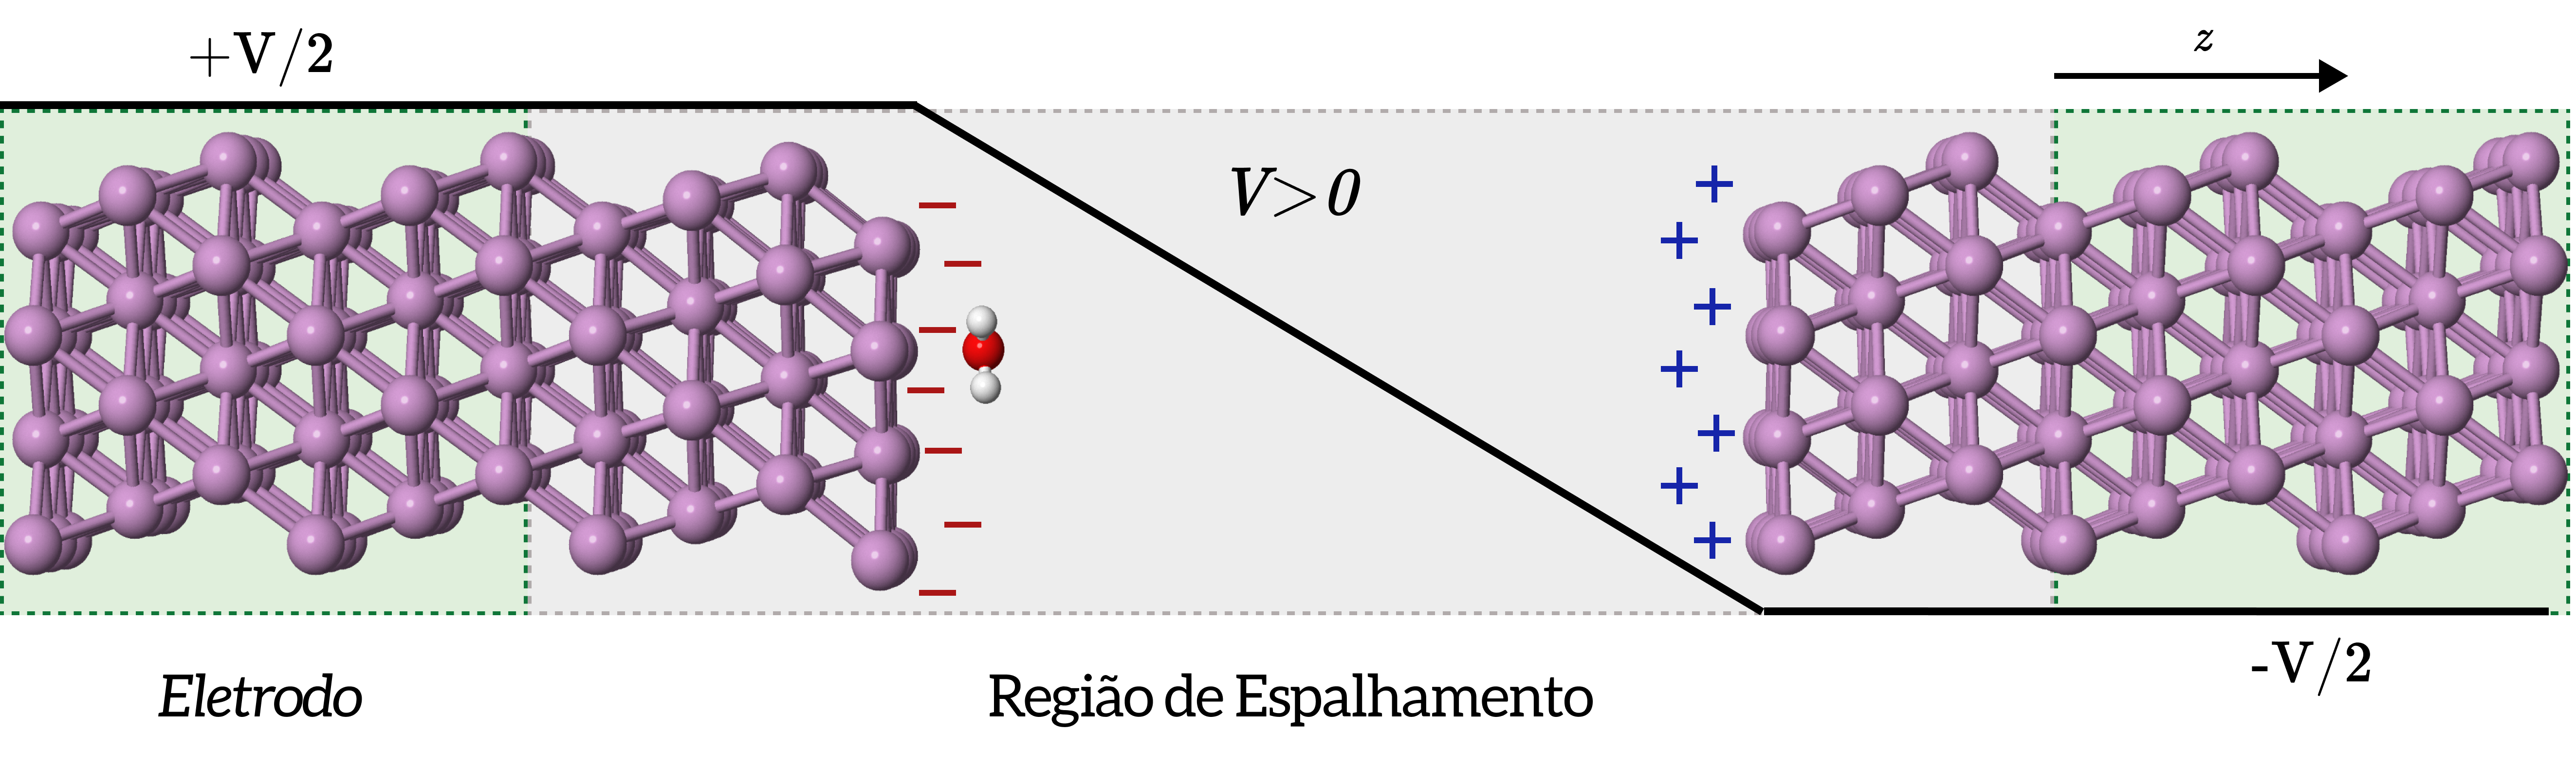
\includegraphics[scale=0.35]{figs/sistema_pd.png}
	\legend{Fonte: compilação da autora.}
\end{figure}

Para aplicar a diferença de potencial externa, primeiramente, determinou-se a geometria de mínima energia utilizando condições periódicas de contorno e em seguida o sistema foi minimizado com o $ V=0.0\,\si{\eV} $ (\textit{potencial 0}). Após a minimização com PBC obteve-se para o funcional PBE $d_{O-Pd}=2.47\,\si{\angstrom} $ e $ \alpha=-4\si{\degree} $ e para o funcional VDW-BH $d_{O-Pd}=2.39\,\si{\angstrom} $ e $ \alpha=2\si{\degree} $. Esses valores coincidem com os obtidos a partir da minimização com \textit{potencial 0}: $d_{O-Pd}=2.46\,\si{\angstrom} $ e $ \alpha=-4\si{\degree} $ para o PBE e $d_{O-Pd}=2.39\,\si{\angstrom} $ e $ \alpha=2\si{\degree} $ para o VDW-BH. Em seguida, com a geometria obtida a partir da otimização com o \textit{potencial 0}, aplicou-se a diferença de potencial entre -2.5 a 2.5 eV com intervalos de 0.5 eV. Com isso, foi possível analisar possíveis transferências de carga através das diferenças de densidade de carga $ \Delta\rho_{V} $ entre o potencial aplicado $ \rho_{V\neq0} $ e $ \rho_{V=0} $. %A análise de diferença de carga foi feita para ambos funcionais (Figura \ref{fig:pd_zcharge}). 

Através do gráfico de $ \Delta\rho_{V} $, percebe-se que a aplicação do potencial externo induz uma pequena transferência de carga entre o metal e a molécula de água (Figura \ref{fig:pd_densidade} e \ref{fig:pd_zcharge}). Além disso, a maior parte dessa diferença está concentrada no átomo de oxigênio e é proporcional ao potencial aplicado. Embora os gráficos de $ \Delta\rho_{ _{+V}} $ e $ \Delta\rho_{ _{-V}} $ sejam semelhantes, observa-se que a flutuação entre essas densidades de carga são assimétricas, ou seja, o efeito do potencial positivo sobre a molécula de água é diferente do negativo (última coluna da Figura \ref{fig:pd_densidade}). Em particular, tem-se que para os potenciais menores ocorre uma flutuação positiva, indicando que nesses casos a interação da molécula com o metal é maior para o potencial positivo. Além disso, observa-se uma polarização de carga superficial na região acima do eletrodo metálico. 

\begin{figure}[t!]
	\centering
	\caption{Variação da densidade de carga dos potenciais aplicados em comparação ao potencial de potencial 0 $ \Delta\rho_{_ {V}}=\rho_{V}-\rho_{0} $ com o funcional PBE. Em todos os recortes foram utilizados o valor de isosuperfície $ 1.80\times10^{-4}\;\si{e}/\si{\angstrom}^3  $ para $ \Delta\rho_{_ {V}} $. Na última coluna está representado a flutuação de densidade de carga entre os potenciais positivos e negativos $ \Sigma\Delta\rho_{_ {V}}=\Delta\rho_{ _{+V}}+\Delta\rho_{ _{-V}} $, onde o valor de isosuperfície é $ 1.67\times10^{-5} \;\si{e}/\si{\angstrom}^3 $. Em todos os casos, azul/vermelho indica uma deficiência/excesso de elétrons.}
	\label{fig:pd_densidade}
	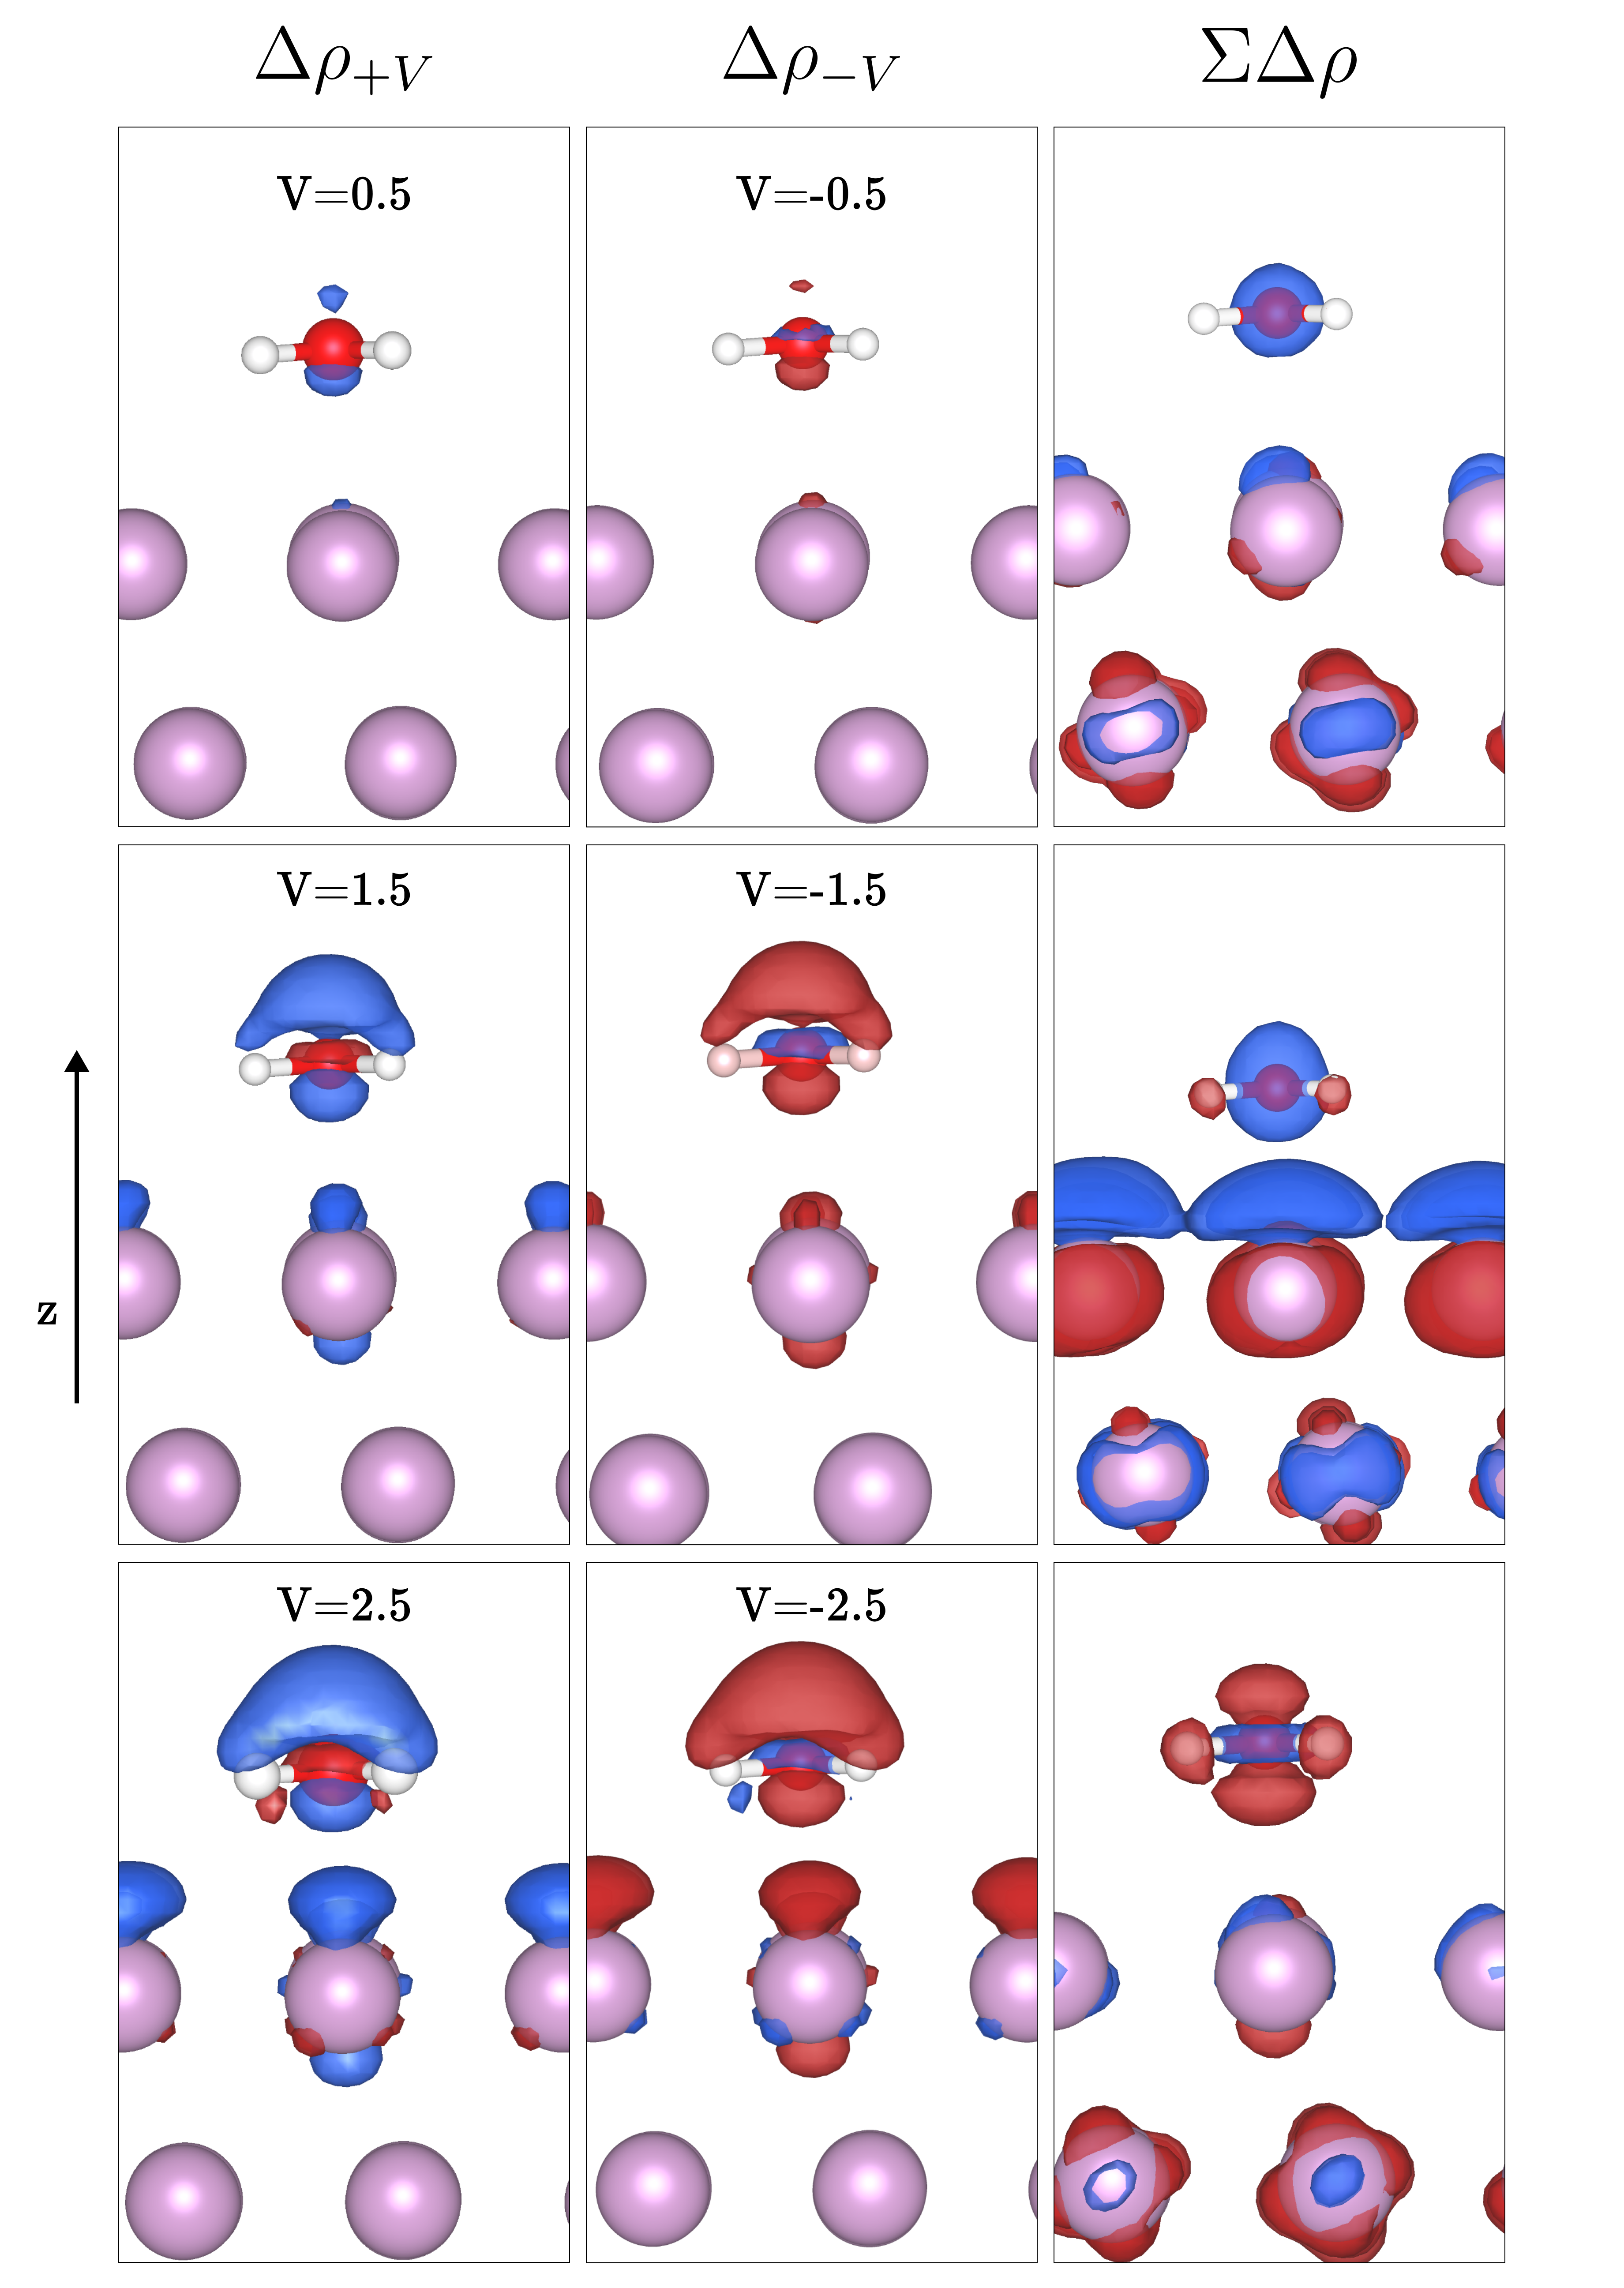
\includegraphics[scale=0.068]{figs/pd_densidade2.png}
	\legend{Fonte: compilação da autora.}
\end{figure}

Considerando as correções com o funcional VDW-BH nos sistemas sem perturbações externas, vimos que as energias de adsorção aumentaram e as propriedades vibracionais foram afetadas. Assim, com o intuito de determinar o efeito das forças de dispersão considerando perturbações externas, comparamos qualitativamente $ \Delta \rho_{V} $ entre os dois funcionais (Figura \ref{fig:pd_zcharge}). Em relação ao funcional VDW-BH, observou-se um comportamento similar ao do PBE através do gráfico de $ \Delta \rho_{V} $ médio ao longo do eixo z para os potenciais $ V=\pm1.5\,\si{\eV}$ e $ V=\pm2.5\,\si{\eV} $ . Ademais, as propriedades geométricas obtidas com a minimização a $ V=0\,\si{eV} $ para os funcionais PBE e VDW-BH, tais como distância $ d_{O-Pd} $ e inclinação $ \alpha $, diferem entre si por $ 0.07\,\si{\angstrom} $ e $ 6\si{\degree} $, respectivamente -- Tabela \ref{tab:neq_geometria_pd}. No entanto, essas variações são similares às obtidas sem perturbações externas (Tabela \ref{tab:geom_pbe} e Figura \ref{fig:neq_pd_mon_freq}). Assim, as ligações responsáveis pelas interações água/Pd na presença dos potenciais externos aqui aplicado não foram significativamente modificadas pela presença do funcional VDW-BH. Esse comportamento também foi observado por \citeauthor{artigo-luana} ao estudar as forças resultantes sobre a molécula de água adsorvida em Au(111) com o funcional VDW-DRSLL$ ^{PBE} $. 


\begin{figure}[t!]
	\centering
	\caption{Comparação da diferença de densidade de carga média ao longo do eixo z dos cálculos com os funcionais PBE e VDW-BH. As densidades foram obtidas nas geometrias correspondentes a cada funcional com os potenciais aplicados $V=\pm 1.5\,\si{\eV} $ e $V=\pm2.5\,\si{\eV}$. As linhas sólidas verticais indicam as respectivas posições dos átomos de Pd abaixo da molécula de água e do átomo de O.}
	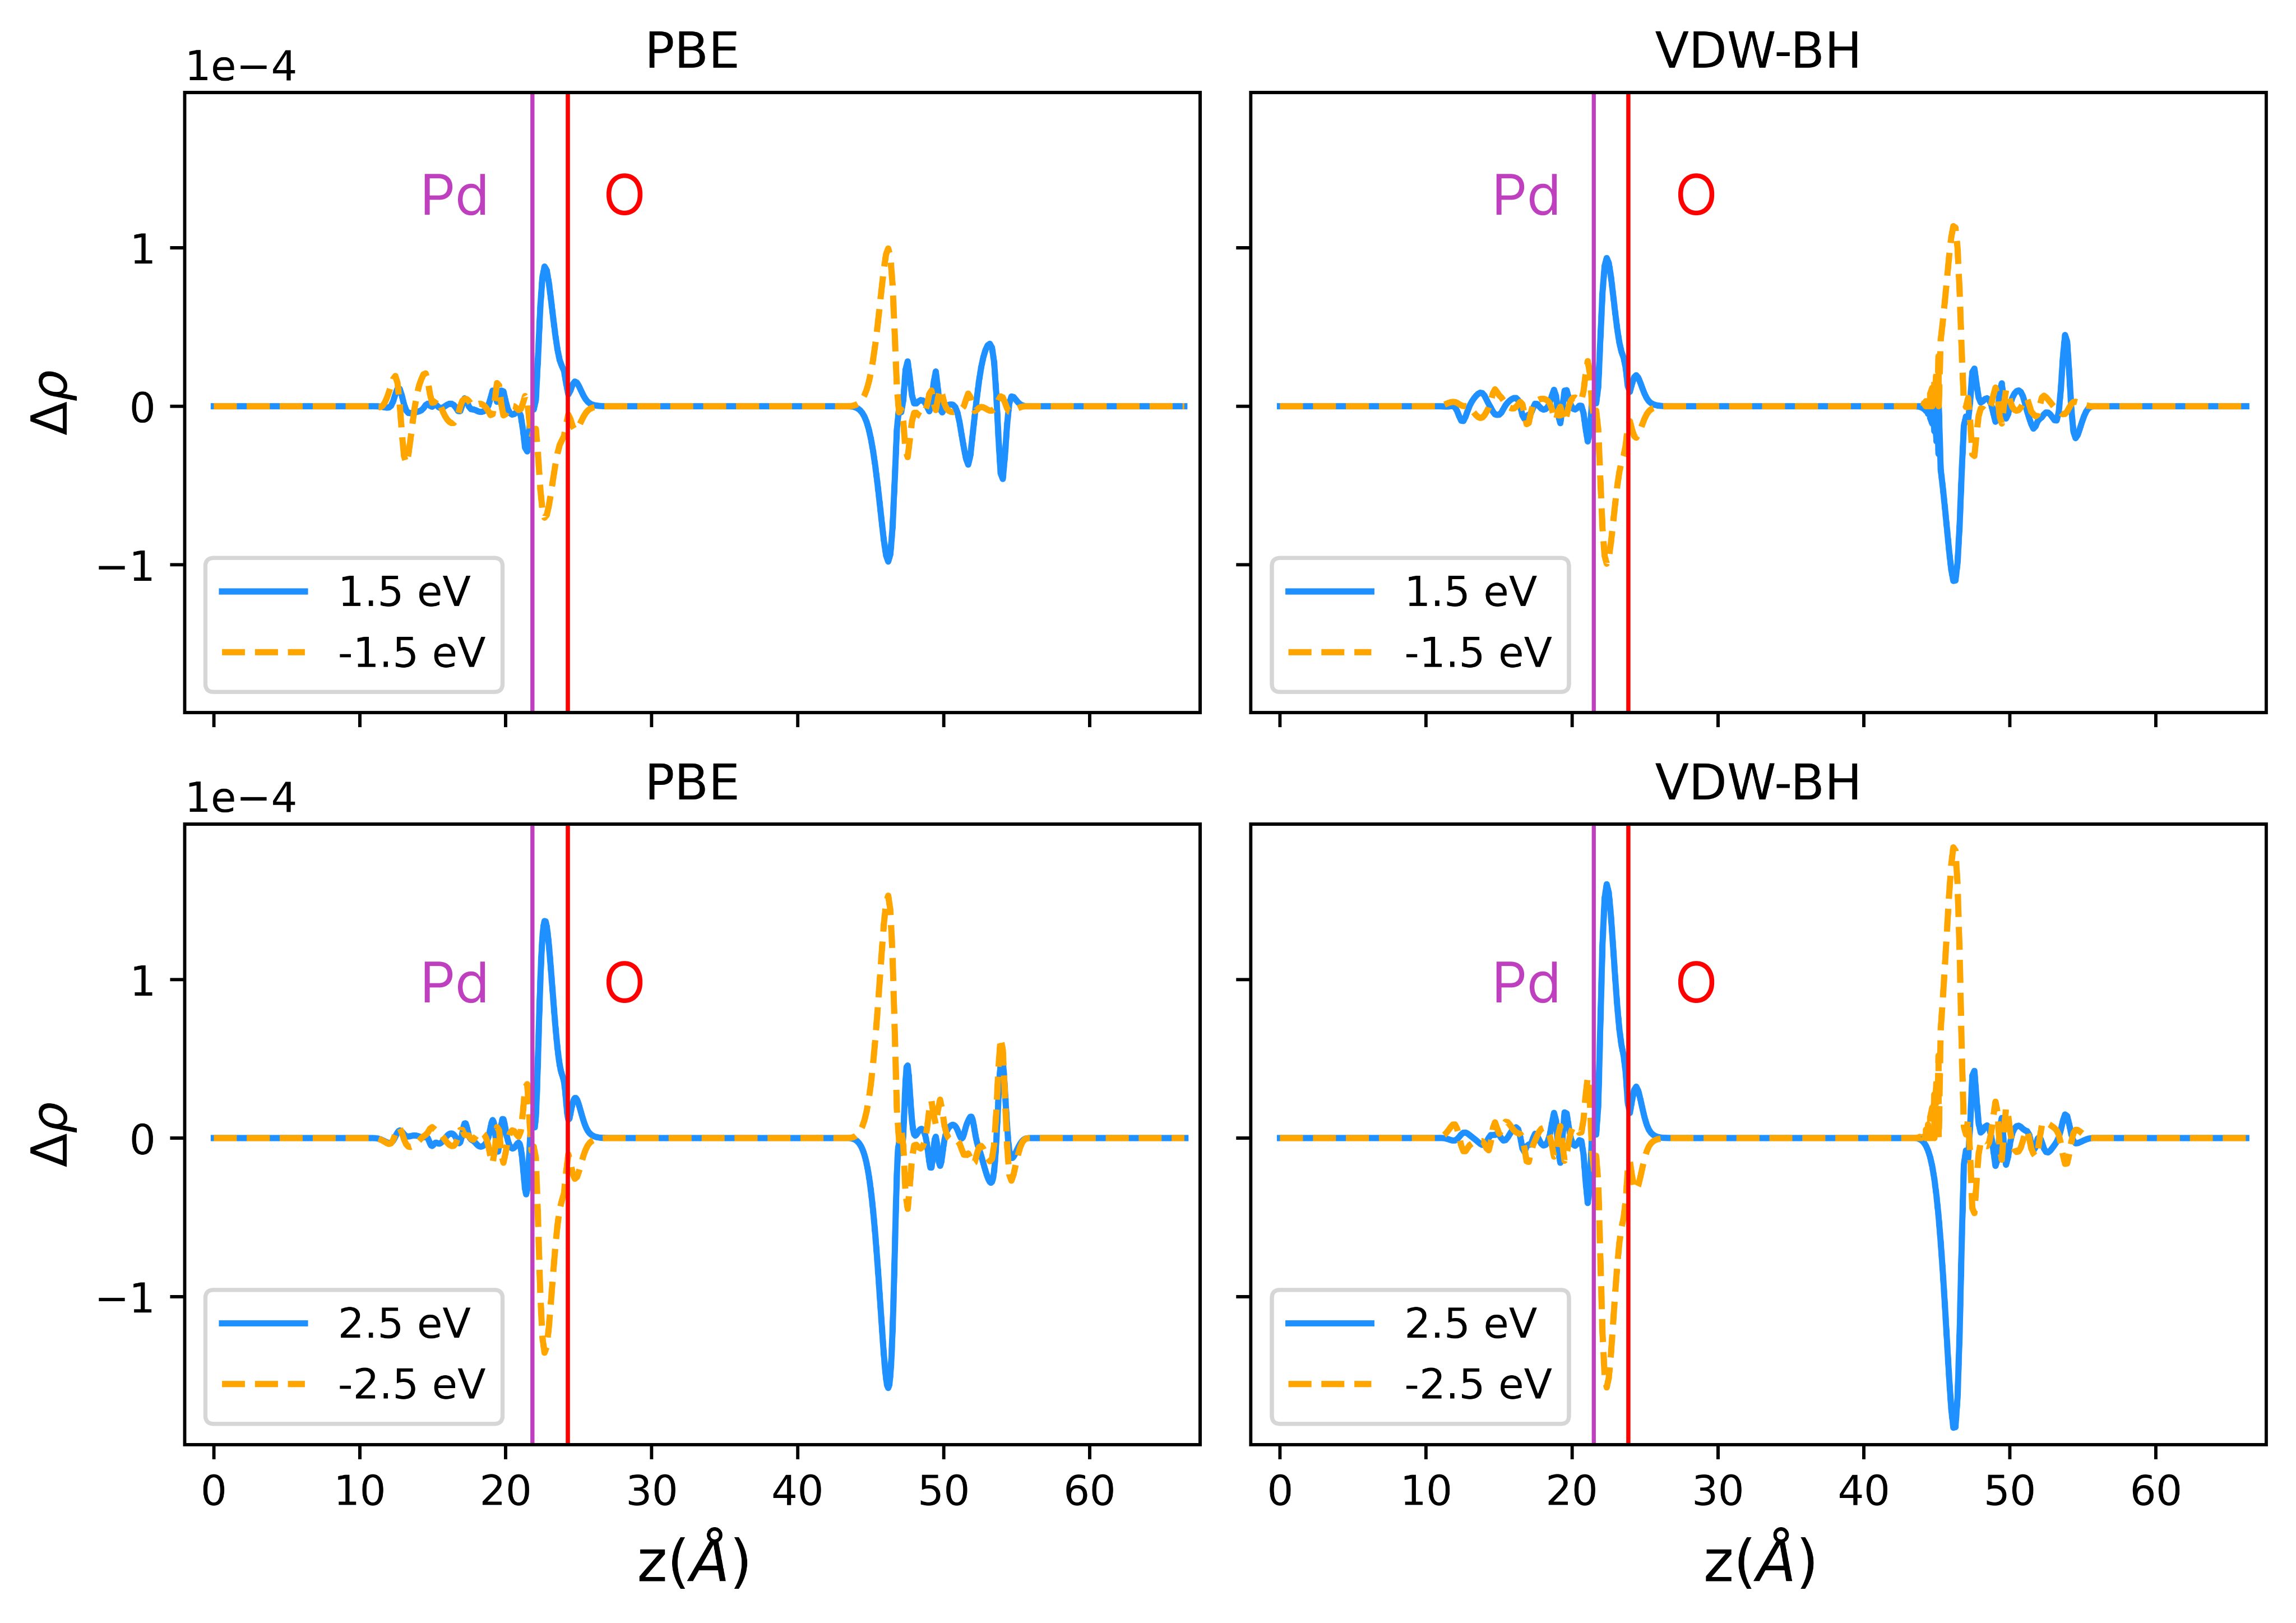
\includegraphics[scale=0.1]{figs/pd_densidade.png}
	\label{fig:pd_zcharge}
	\legend{Fonte: compilação da autora.}
\end{figure}

Tendo em vista que a utilização de correções do tipo vdw não afeta significativamente a descrição do sistema ao aplicar o intervalo de potenciais externos aqui utilizados, então foi realizado a minimização das coordenadas para $ V\neq0 $ utilizando o funcional PBE. Isso permitiu obter as propriedades geométricas (Tabela \ref{tab:neq_geometria_pd} e Figura \ref{fig:neq_pd_mon_geo}) e calcular as frequências dos modos normais de vibrações (Tabela \ref{tab:neq_freq_pd} e Figura \ref{fig:neq_pd_mon_freq}) considerando uma diferença de potencial externa, bem como definir o efeito resultante sobre a ligação água/metal.
\begin{table}[h!]
	\centering
	\caption{Variação das propriedades geométricas da molécula de água adsorvida no Pd(111) em relação ao potencial externo aplicado V obtidas a partir da otimização com o funcional PBE. As propriedades incluem a distância entre o átomo de O e Pd ($d_{O-Pd}(\si{\angstrom})$), o deslocamento lateral ($\Delta Oxy$), a inclinação ($\alpha$), a distância entre os átomos de H e O ($d_{O-H}(\si{\angstrom})$) e o ângulo ($\Theta$) entre os átomos de H. A última linha refere-se à relaxação a 0 bias com o funcional VDW-BH. \label{tab:neq_geometria_pd}}
	\begin{threeparttable}
		\begin{tabular}{Sccccc} 
			\hline\hline\addlinespace[3.6pt]
			\multicolumn{6}{c}{\textbf{Propriedades Geométricas $ H_2O/Pd$}}   \\\midrule
			{V (\si{eV})}   &{$d_{O-Pd}(\si{\angstrom})$} & {$ d_{O-H}(\si{\angstrom})$}  & {$\Delta\, Oxy(\si{\angstrom})$} &{$\Theta(\si{\degree})$}&{$\alpha(\si{\degree})$}\\
			\hline
			2.50		&2.56	&0.98	&0.67	&103&-22 \\
			2.00		&2.53	&0.98	&0.60   &103&-17 \\
			1.50		&2.51	&0.98	&0.55	&103&-13 \\
			1.00		&2.49	&0.98	&0.55	&103&-10\\
			0.50		&2.48	&0.98		&0.49	&102&-6\\
			0.00		&2.46	&0.98	&0.49	&104&-4\\
			-0.50		&2.45	&0.98	&0.43	&104&0 \\
			-1.00		&2.44	&0.98&0.42	&104&3 \\
			-1.50		&2.43		&	0.98/0.97	&	0.38	&104	& 6\\
			-2.00		&2.42	&0.97	&0.26	&104&12 \\
			-2.50		&2.41	&0.97	&0.24	&104&16 \\	
			\midrule
			{0.00}\tnote{$\dagger$} 	&2.39	&0.98	&0.35	&104&2\\%\\{PBC}&2.47&0.98&0.49&104&-4\\		
			\hline\hline
		\end{tabular}
		\begin{tablenotes}\footnotesize
			\item[$\dagger$] Funcional VDW-BH
		\end{tablenotes}
	\end{threeparttable}
	\legend{Fonte: compilação da autora.}
\end{table}

\begin{figure}[h!]
	\centering
	\caption{Variação da inclinação $ \alpha $ e da distância $ \Delta d_{O-Pd} $ de acordo com o potencial externo aplicado. O valor de $ \Delta d_{O-Pd}=d_{O-Pd,V}-d_0 $ mensura o quanto a molécula se afastou em relação à posição inicial $ d_0=2.46\,\si{\angstrom} $. Além disso, também estão ilustrados as posições do monômero em relação à superfície metálica.}
	\label{fig:neq_pd_mon_geo}
	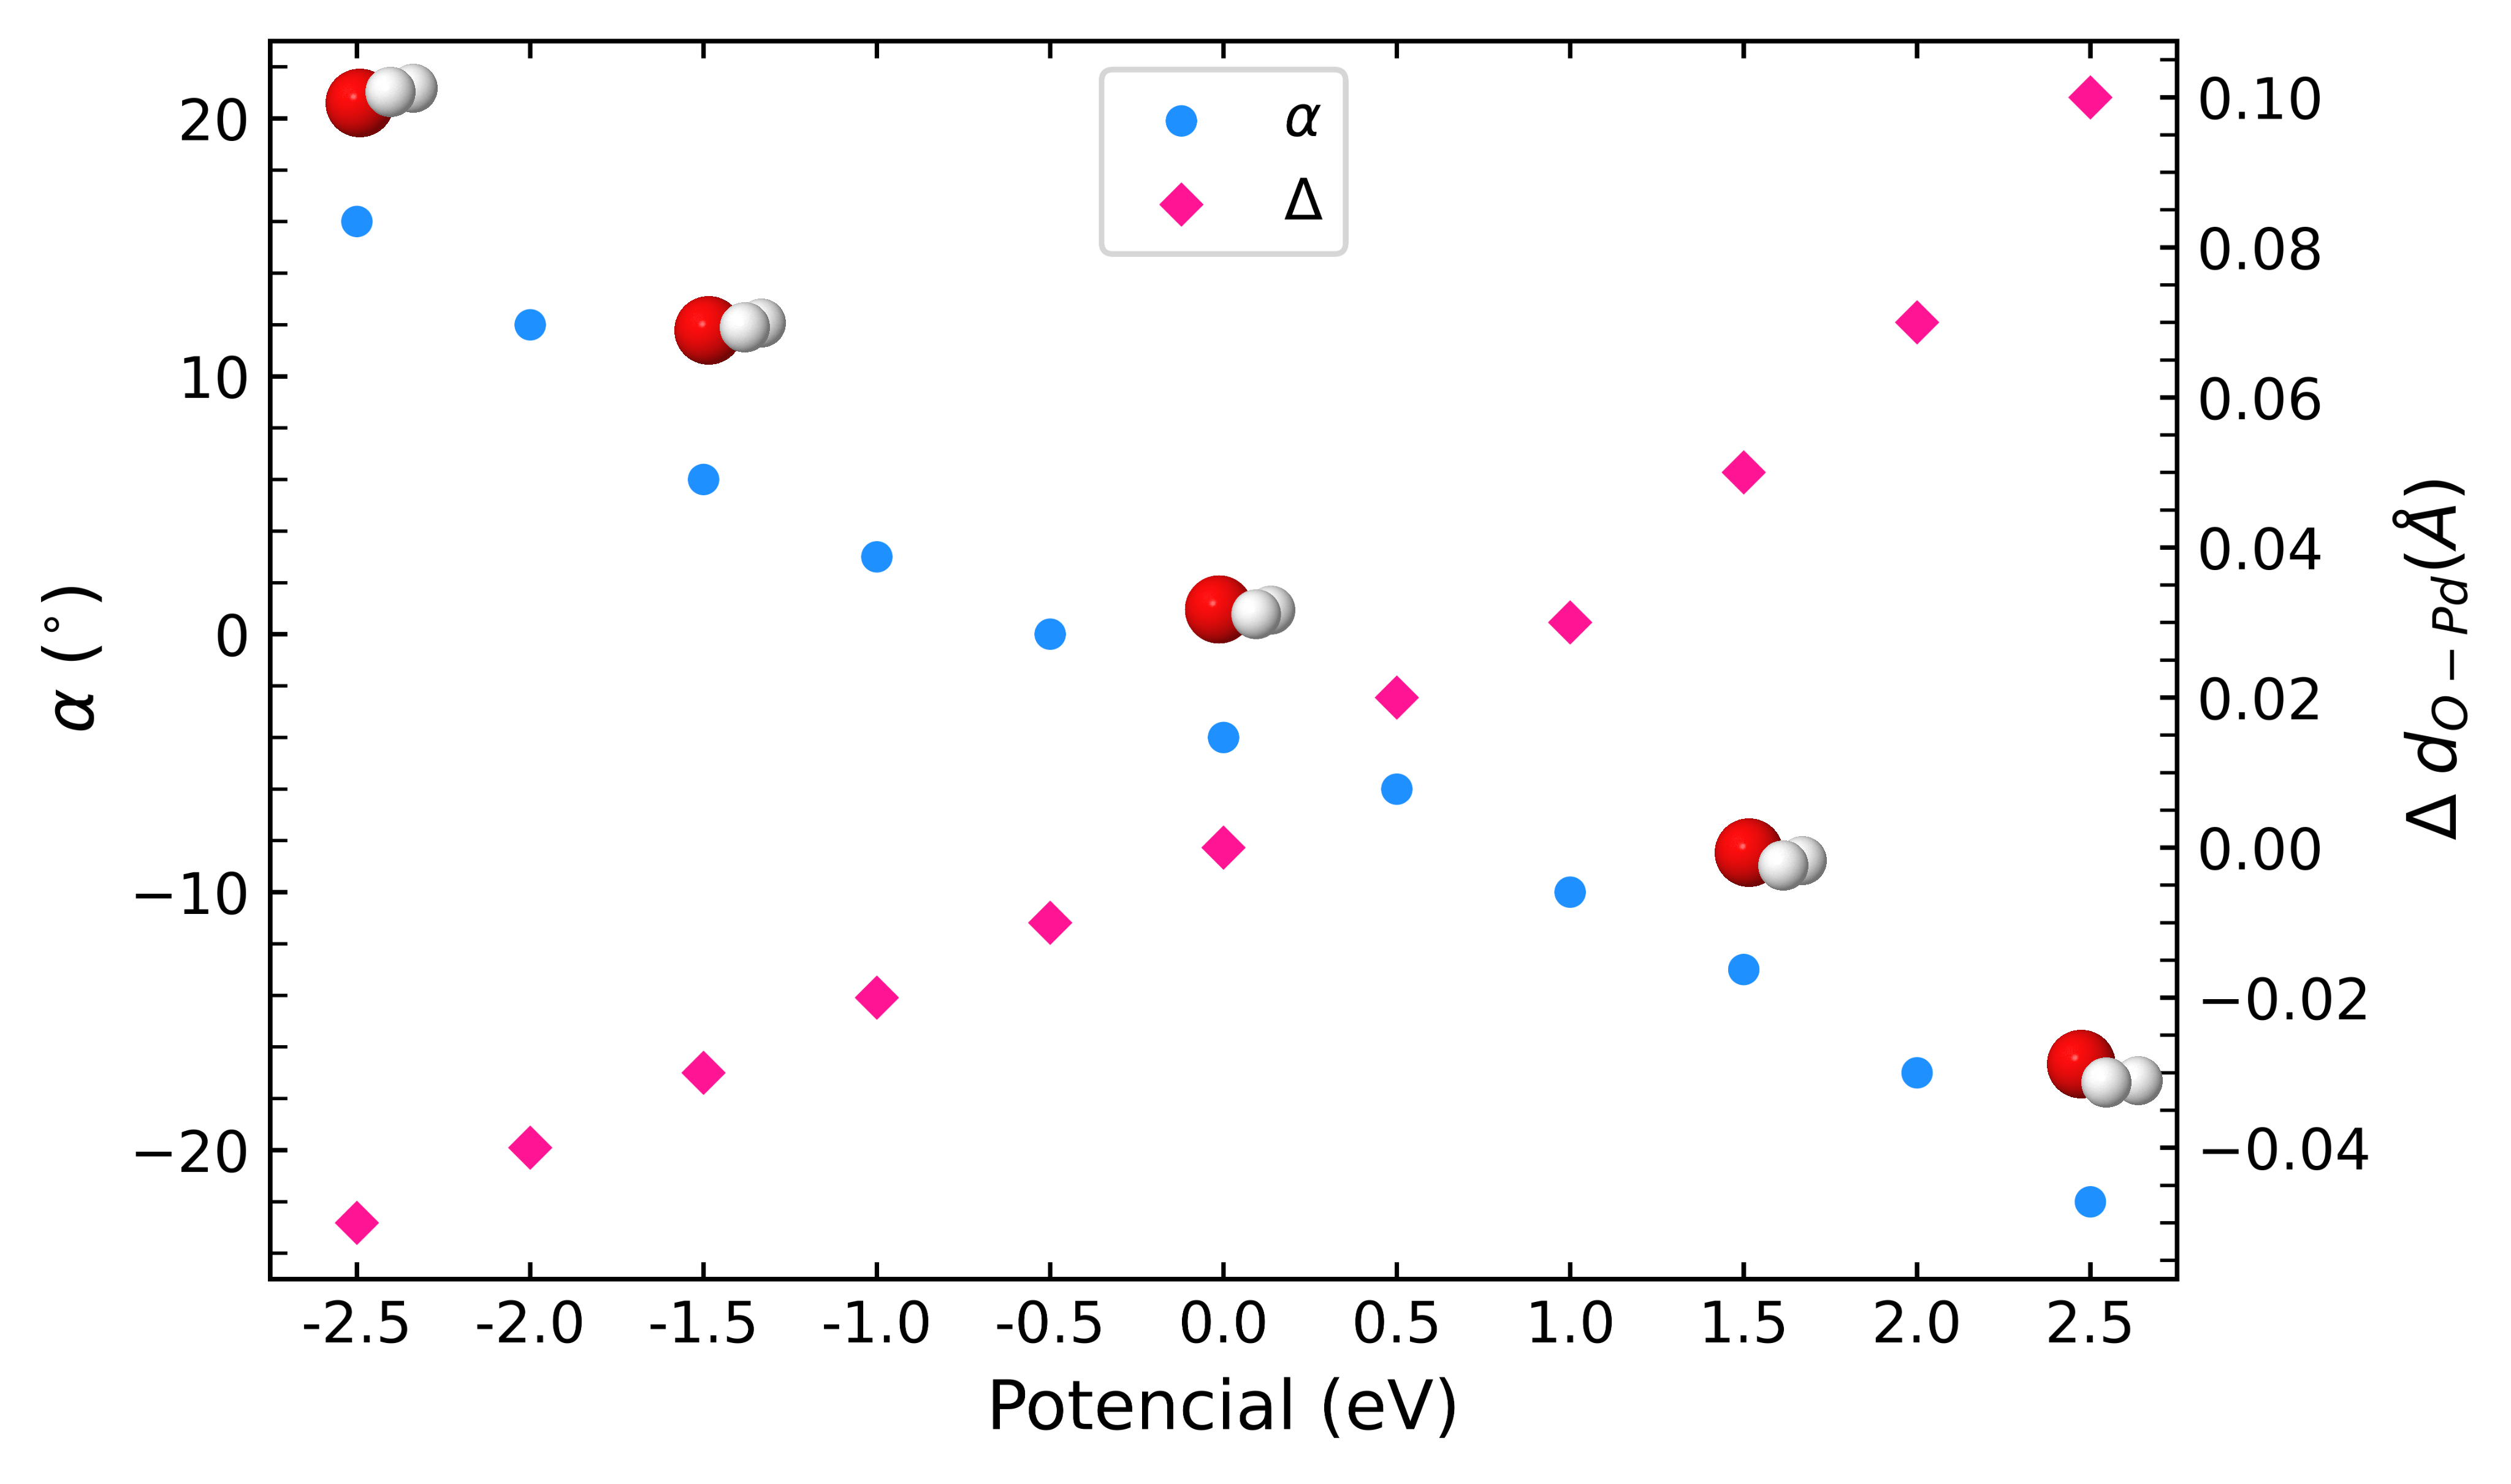
\includegraphics[scale=0.088]{figs/monomero_pd_ang.png}
	\legend{Fonte: compilação da autora.}
\end{figure}

Sem a presença de perturbações externas, a interação água/metal ocorre através da interação do orbital $ b_1 $ com os níveis vazios do Pd. No entanto, ao aplicar uma diferença de potencial ao sistema, a interação resultante vai ser uma combinação do efeito eletrostático e da interação água/metal. Assim, analisando o efeito dessa combinação, nota-se uma tendência da molécula de se aproximar do metal para $ V<0 $ e de se afastar do metal para $ V>0 $ (Figura \ref{fig:neq_pd_mon_geo}). Isso ocorre devido à polarização de carga superficial negativa/positiva no metal que surge ao aplicar um potencial positivo/negativo sobre o eletrodo metálico. O efeito dessa polarização aparece nos gráficos de densidades de carga, no qual, acima da superfície, tem-se uma concentração de densidade de carga representando a deficiência/excesso de elétrons (Figura \ref{fig:pd_densidade}). 

Dessa forma, essa polarização superficial afeta a interação eletrostática entre o metal e a molécula de água, ora atraindo-a, ora repelindo-a. Logo, para $ V>0 $ ocorre um aumento máximo de $ 0.1\,\si{\angstrom} $ da distância $ d_{O-Pd} $ e uma redução máxima de $ -18\si{\degree} $ da inclinação da molécula de água $ \alpha $, ao passo que para $ V<0 $ o átomo de O é atraído para a superfície metálica em até de $ 0.05\,\si{\angstrom} $ e rotaciona em até $ 20\si{\degree} $. É possível notar que as mudanças em $d_{O-Pd}$ e $\alpha$ dependem do sinal de V, em concordância com o comportamento assimétrico observado nos gráficos de $\Delta\rho_{V}$. Assim, esse comportamento assimétrico está relacionado às alterações estruturais que ocorrem nas moléculas de água, visto que a molécula de água altera a sua orientação e consequentemente, a interação entre a água e o metal são alteradas. Portanto, o sinal do potencial aplicado afeta o comportamento da molécula de água e a interação com o metal.

% que afetam o \textit{overlap} entre os orbitais da molécula de água e os da superfície



Além do efeito eletrostático sobre a interação água/metal, observa-se também, como resultado da aplicação do potencial externo alterações na repulsão de Pauli. Para definir a contribuição dessa interação, \citeauthor{artigo-luana} separaram a contribuição do campo elétrico das demais interações e associaram o efeito resultante da interação água/metal ao aumento (diminuição) da repulsão de Pauli. Dessa forma, a combinação desses efeitos afetam diretamente a interação água/metal e consequentemente definem a orientação da molécula de água sobre a superfície carregada. Além disso, esses efeitos são capazes de alterar a reatividade e as propriedades de adsorção do metal, como pode ser visto pela variação proporcional do deslocamento xy ($ \Delta Oxy $) em relação ao aumento/redução de V. Isso mostra que o potencial externo afeta também o sítio de adsorção preferencial da molécula de água.
\begin{table}[h!]
	\centering
	\caption{Frequências dos modos normais de vibrações do monômero adsorvido no Pd(111) de acordo com o potencial externo aplicado (V).}
	%\begin{threeparttable}
	\begin{tabular}{Sccc} 
		\hline\hline\addlinespace[3.6pt]
		\multicolumn{4}{c}{\textbf{Frequências dos Modos Normais $ H_2O/Pd\,(\mathbf{\si{\cm}^{-1}})$}}\\ \midrule
		{V (eV)}   &{Bending}	&{Stretching(S)}	&{Stretching(AS)}\\
		\hline			
		2.5		&1612	&3563	&3638\\
		2.0		&1613	&3575	&3662\\
		1.5		&1613	&3608	&3683\\
		1.0		&1612	&3594	&3686\\
		0.5		&1611	&3608	&3693\\
		0.0		&1608	&3609	&3696\\
		-0.5		&1618	&3629	&3725\\
		-1.0		&1618	&3635	&3733\\
		-1.5		&1623	&3641	&3741\\
		-2.0		&1624	&3654	&3757\\
		-2.5		&1628	&3664	&3766\\
		\midrule	
		{PBC} 		&1600&3574&3668	\\
		\hline\hline
	\end{tabular}
	\legend{Fonte: compilação da autora.\label{tab:neq_freq_pd}}
\end{table}
\begin{figure}[h!]
	\centering
	\caption{Frequências fundamentais do monômero adsorvido no Pd(111)) de acordo com o potencial externo aplicado. As linhas pontilhadas correspondem aos valores experimentais do monômero isolado.}
	\label{fig:neq_pd_mon_freq}
	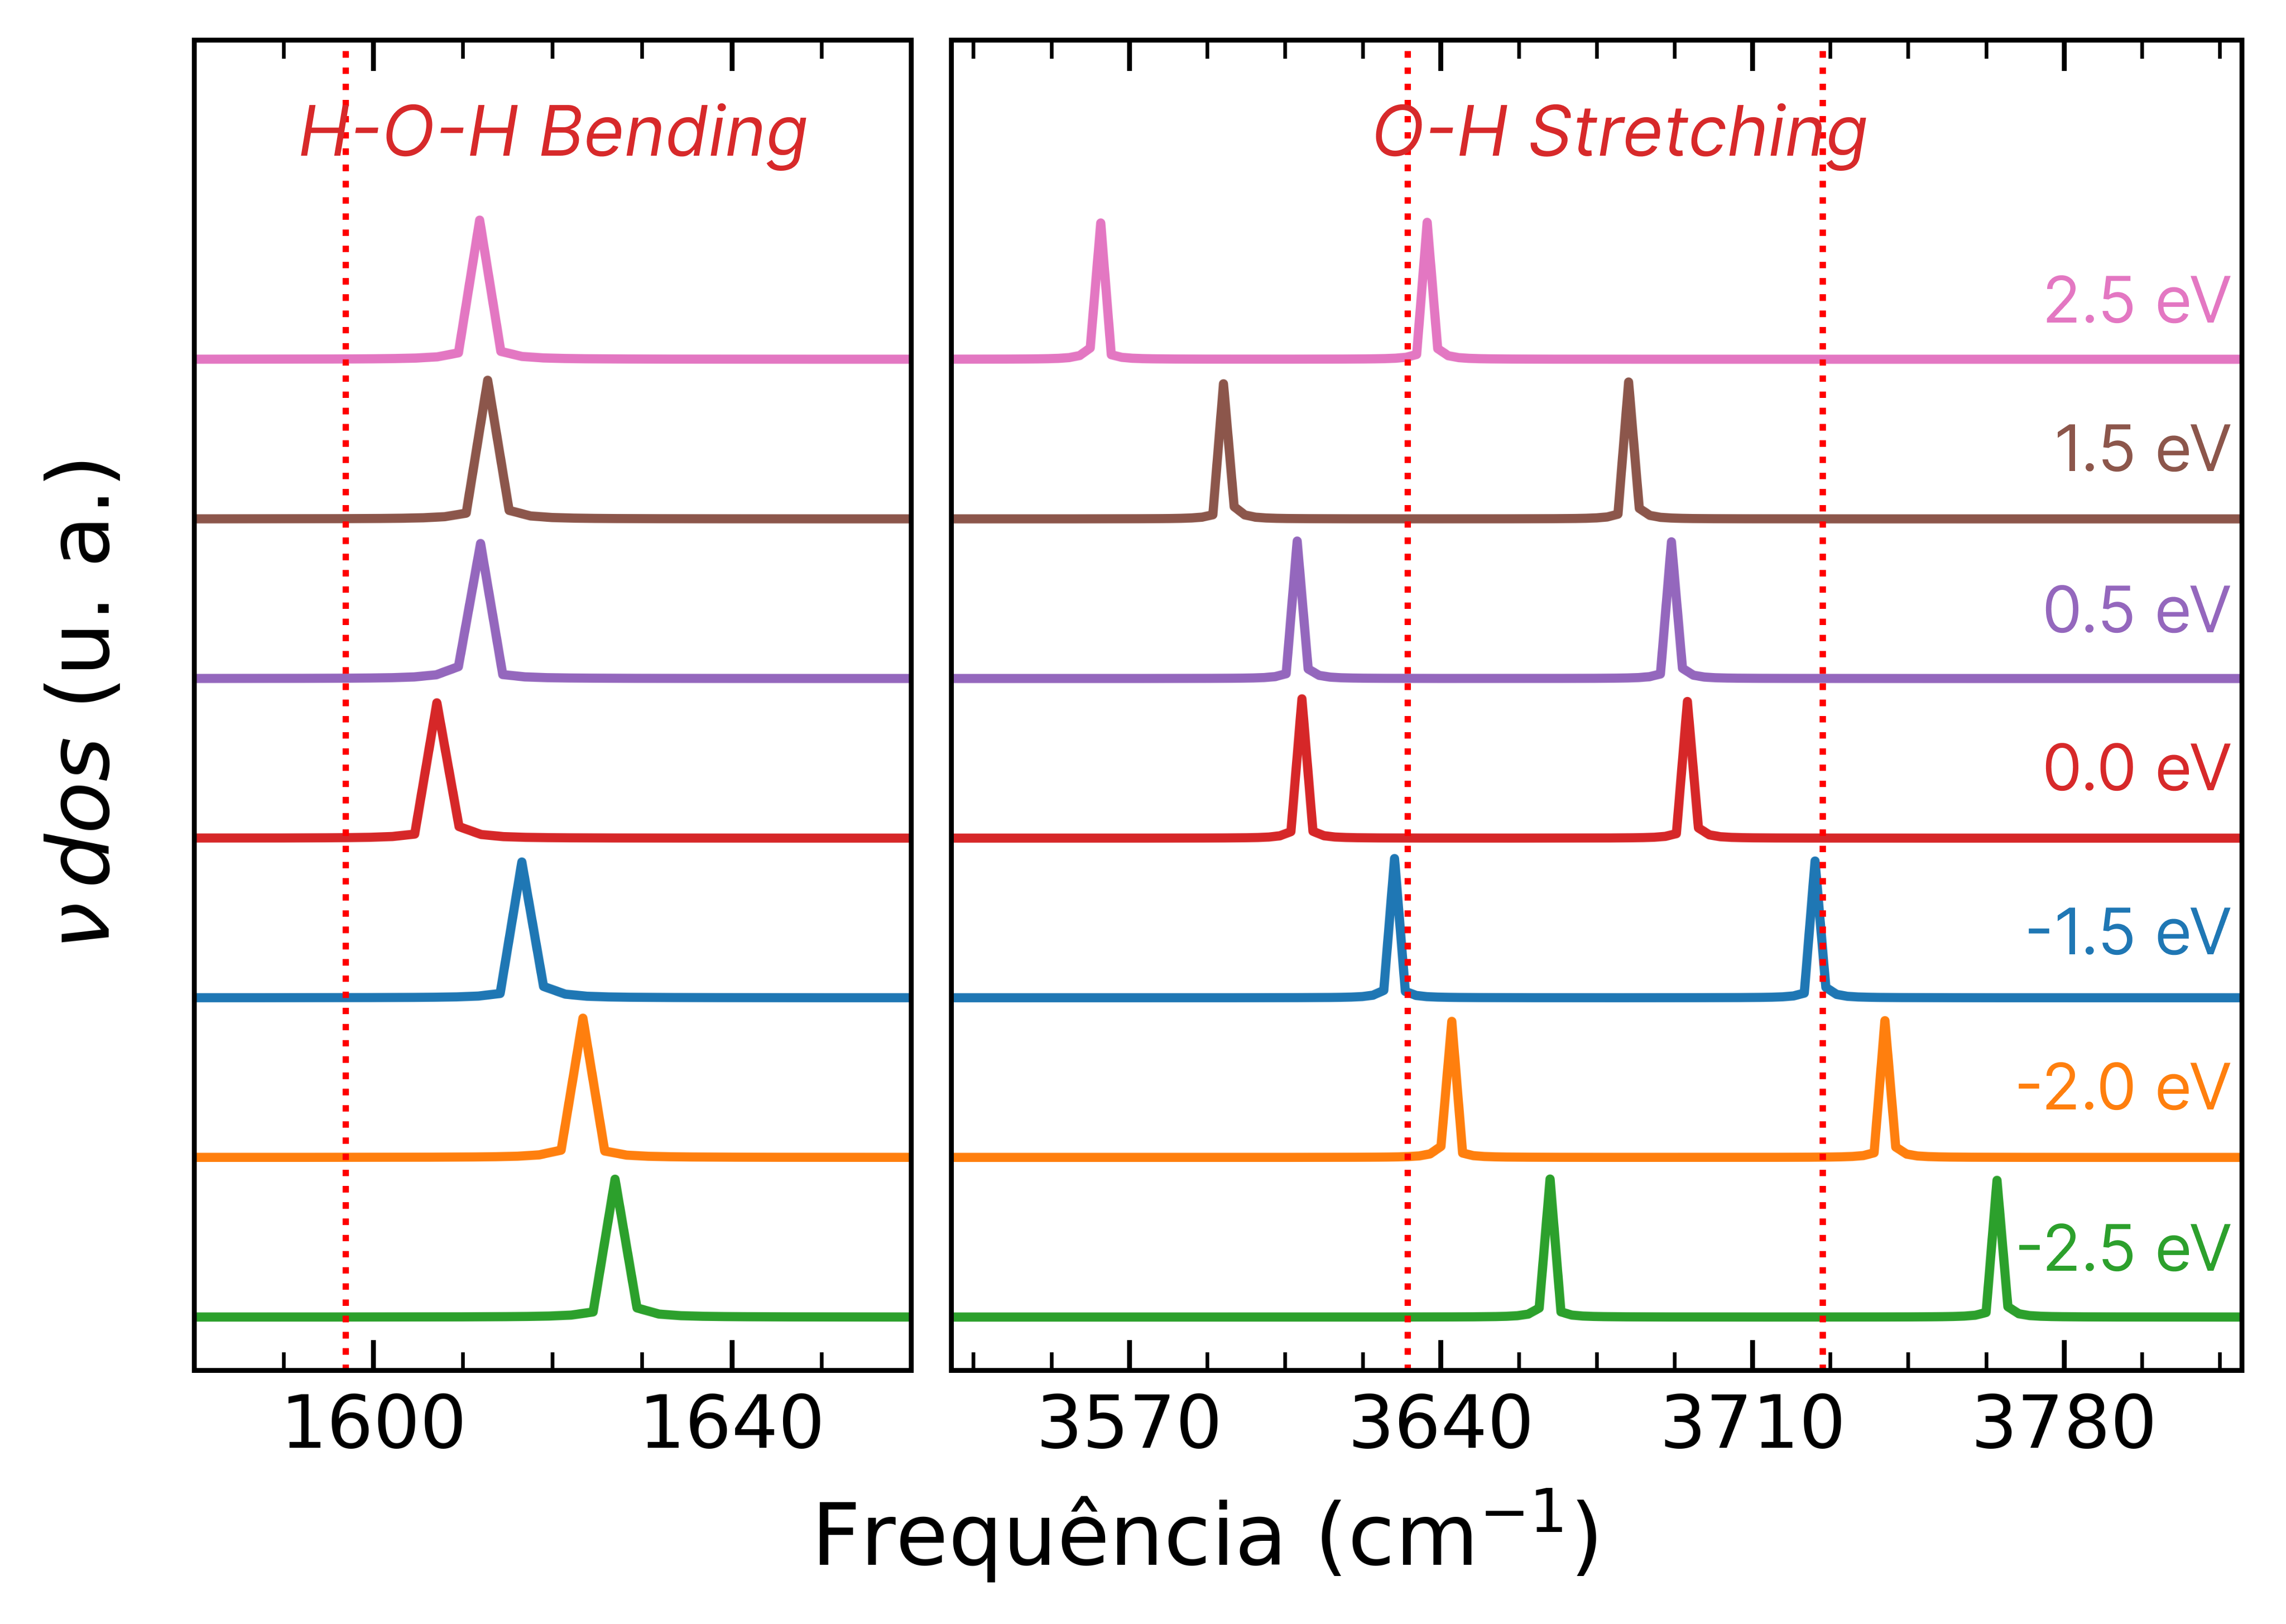
\includegraphics[scale=0.08]{figs/freq_monomer_pd.png}
	\legend{Fonte: compilação da autora.}
\end{figure}

As alterações estruturais provocadas pela diferença do potencial externo refletem nas frequências dos modos vibracionais (Tabela \ref{tab:neq_freq_pd} e Figura \ref{fig:neq_pd_mon_freq}). Tais alterações incluem a repulsão/atração da molécula de água em direção ao metal e o fato do eletrodo ser tratado como semi-infinito e não finito. Esse último ponto é visto pela diferença nas frequências obtidas com o sistema completo (Figura \ref{fig:sistema_pd}) com condições periódicas de contorno (\textit{periodic boundary conditions}- PBC), em relação ao slab de tamanho $ 6\times4\times4 $ camadas -- Tabela \ref{tab:modos}. Assim, houve uma diminuição média de $ \sim 75\;\si{\cm}^{-1} $ nas frequências de \textit{stretching} ao aumentar o número de camadas (4 para 10) e diminuir o tamanho do plano xy ($ 6\times4 $ para $ 3\times4 $). Essa variação é resultado do efeito eletrostático da molécula de água com as células vizinhas ao diminuir o tamanho da célula unitária, uma vez que ao tratar os eletrodos como semi-infinitos a variação foi de $ \sim 30\;\si{\cm}^{-1} $ nas frequências de \textit{stretching}. No entanto, devido ao custo computacional de um cálculo NEGF, aumentar o tamanho do plano metálico se torna inviável.  


Ao variar o potencial externo aplicado, as frequências diminuem com o aumento do potencial para V>0 variando $ 58\,\si{cm}^{-1} $ para $ V=2.5\,\si{\eV} $; quando o potencial diminuiu, as frequências aumentam até $ 70\,\si{cm}^{-1}$ para $ V=-2.5\,\si{\eV} $. Essas alterações refletem a rotação da molécula devido à superfície carregada, que por sua vez, intensificam ou enfraquecem as ligações O-H. Assim, para potenciais positivos, a molécula se liga mais fortemente ao metal através da interação entre os átomos de H e a superfície negativamente carregada. Por outro lado, para potenciais negativos, os átomos de H se afastam da superfície carregada positivamente e assim, interagem menos com o metal.

%Por fim, tem-se que a aplicação do potencial externo altera as propriedades estruturais e vibracionais da molécula adsorvida no Pd. Em particular 


O modelo estudado constitui um protótipo da interação água/metal e não inclui ligações de hidrogênio que são determinantes nas ativações de processos de oxidação e redução da molécula de água em superfícies metálicas carregadas \cite{bias-pd}. Além disso, através do cálculo de forças fora do equilíbrio foi possível realizar a otimização da geometria que determinou a posição de mínima energia e que revelaram alterações vibracionais e estruturais. Assim, não observou-se processos de oxidação ou redução do monômero na superfície metálica, pois essas reações resultam do balanço entre as interações da água com a superfície carregada e interações entre as moléculas de água da interface e as moléculas de água de camadas superiores \cite{pd_bias_exp,pd_bias_exp2,pd_bias_exp3}. %Assim, os resultados acima discutidos  ao se aplicar um potencial externo, todavia, não considerou o efeito sobre as ligações de hidrogênio. 

%Além disso, nossos resultados estão em concordância com resultados teóricos que revelaram o comportamento dependente do potencial das moléculas de água na superfície de Pd \cite{bias-pd}. Ademais, encontrou-se que o processo de redução ocorre através da dissociação da água e formação de hidretos na superfície e é ativado pela interação com o metal a 0.5 V. Por outro lado, a oxidação ocorre a 1.1 V através da formação de hidróxido na superfície e com transferência de prótons para as moléculas das camadas superiores. De acordo com os autores, a posição de equilíbrio da solução aquosa e processos de redução/oxidação resultam do balanço entre as interações da água com a superfície carregada e interações entre as moléculas de água da interface e as moléculas de água de camadas superiores. 
 



\section{Ouro\label{sec:au_negf}}

%Para a superfície metálica de Au(111) foram estudados dois sistemas protótipos: monômero e camada de água. O primeiro inclui apenas a interação água/metal (Seção \ref{sec:neq_au_mon}), ao passo que o segundo inclui tanto interações água/metal como ligações de hidrogênio entre água (Seção \ref{sec:neq_au_layer}).% Além disso, a camada representa um modelo da interface água líquida/metal. %Vale ressaltar que os eletrodos de Au(111) possuíam menos camadas que os eletrodos de Pd(111). Isso possibilitou estudar a camada de água adsorvida, bem como examinar o comportamento das estruturas com a aplicação de potenciais externos maiores, visto que um cálculo fora do equilíbrio é caro computacionalmente.
\subsection{Monômero \label{sec:neq_au_mon}}
A investigação do potencial externo aplicado à interface água/Au(111) iniciou pela análise do monômero na orientação \textit{flat} adsorvido na superfície metálica de Au(111) com $ 3\times4 $ átomos no plano da superfície. A base atômica localizada que descreve o Au é menor que a base utilizada no Pd (Apêndice \ref{apd:metal} -- Tabelas \ref{tab:raios_corte} e \ref{tab:au}) logo, o eletrodo utilizado possui 3 camadas e a região de espalhamento 4 e 3 camadas de cada lado (Figura \ref{fig:sistema_au}); o parâmetro de rede do Au utilizado foi de $ 4.24\,\si{\angstrom} $ e entre as duas superfícies metálicas havia um vácuo de $ 20\,\si{\angstrom} $, resultando em uma célula unitária de tamanho $ 10.30\times9.90\times53.00\,\si{\angstrom} $. Todas as minimizações foram realizadas com o funcional PBE e o potencial externo aplicado variou entre -5.0 a 5.0 eV, com intervalos entre 1.0 e 1.5 eV. %Para cada otimização, utilizou-se como coordenadas iniciais as obtidas com \textit{potencial 0}.
\begin{figure}[h!]
	\centering
	\caption{Ilustração do sistema utilizado para aplicar a diferença de potencial externa à interface água/Au(111), bem como as regiões correspondentes aos eletrodos e região de espalhamento.}
	\label{fig:sistema_au}
	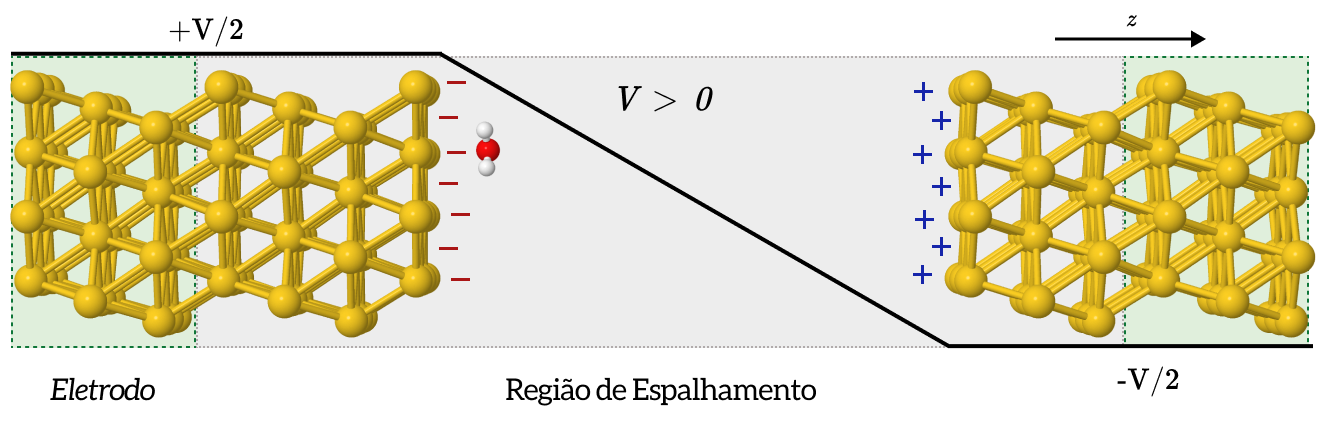
\includegraphics[scale=0.35]{figs/sistema_negf.png}
	\legend{Fonte: compilação da autora.}
\end{figure}

Utilizando condições periódicas de contorno, obteve-se que a energia de adsorção da molécula \textit{flat} adsorvida no Au foi de $ E_{ads-Au}=0.10\,\si{\eV}  $, próxima ao valor de 0.13 eV reportado na literatura com o funcional PW90 \cite{michaedelis}. Após a minimização com PBC obteve-se $d_{O-Au}=2.80\,\si{\angstrom} $ e $ \alpha=-8\si{\degree} $. Essa distância é maior que a distância do monômero adsorvido no Pd $ d_{O-Pd} =2.47 \,\si{\angstrom}$ e está de acordo com os valores obtidos com o \textit{potencial 0}($d_{O-Au}=2.82\,\si{\angstrom} $ e $ \alpha=-10\si{\degree} $). Assim, a molécula se liga fracamente ao Au, sendo portanto, reportado como um metal hidrofóbico \cite{monomer}. 

Analisando as propriedades geométricas da otimização do monômero em função do potencial externo para $ V\neq0 $ (Tabela \ref{tab:neq_au_geo} e Figura \ref{fig:neq_au_mon_geo}), observa-se uma variação significativa da distância a medida que se aumenta o valor de V, onde mesmo para o potencial V=1.5 eV a variação em relação à posição inicial foi de $ \Delta_{d_{O-Au}}=0.52\,\si{\angstrom} $. Em contrapartida, para esse mesmo potencial aplicado ao eletrodo de Pd a molécula se distanciou apenas $ 0.05 \,\si{\angstrom} $. Essa discrepância é resultado da hidrofobicidade do Au e da reatividade do Pd e revela o efeito desses fatores ao se aplicar um potencial externo numa célula eletroquímica.

 

\begin{table}[t!]
	\centering
	\caption{Propriedades geométricas obtidas a partir da otimização da molécula de água adsorvida na superfície metálica de Au(111) de acordo com o potencial V aplicado. As propriedades geométricas analisadas foram a distância entre o átomo de O e Au $d_{O-Au}(\si{\angstrom})$ e entre os átomos de H e de O $ d_{O-H}(\si{\angstrom})$, deslocamento lateral no eixo x e y ($ \Delta Oxy $), ângulo $ \Theta $ entre os átomos de H e inclinação $ \alpha $ em relação à superfície.\label{tab:neq_au_geo}}
	\begin{tabular}{Sccccc} 
		\hline\hline\addlinespace[3.6pt]
		\multicolumn{6}{c}{\textbf{Propriedades Geométricas $ H_2O/Au $ }}   \\\midrule
		{V (eV)}   &{$d_{O-Au}\,(\si{\angstrom}) $}&{$d_{O-H}\,(\si{\angstrom}) $} &{$\Delta\, Oxy \, (\si{\angstrom})$}	&{$\Theta(\si{\degree})$}&{$\alpha(\si{\degree})$}\\
		\hline
		5.0		&3.55	&0.98	&1.56	&101	&-89\\	
		4.0		&3.57	&0.98/0.97	&1.67	&102	&-90\\	
		2.5		&3.49	&0.97	&1.53	&102	&-87\\
		1.5		&3.34	&0.98/0.97	&1.34	&102	&-73\\
		0.0		&2.82	&0.97	&0.49	&104	&-10\\
		-1.5		&2.72	&0.97	&0.07	&104	&25 \\
		-2.5		&2.70	&0.97	&0.13	&104	&36 \\
		-4.0		&2.71	&0.97	&0.28	&104	&53 \\
		-5.0		&2.72	&0.97	&0.48	&104	&66 \\ %\midrule 
	%	PBC		&2.80	&0.97	&0.48	&104	&-8 \\
		\hline\hline
	\end{tabular}
	\legend{Fonte: compilação da autora.}
\end{table}


\begin{figure}[b!]
	\centering
	\caption{Variação da inclinação $ \alpha $ e da distância $ \Delta d_{O-Au} $ em função do potencial externo aplicado V. A distância $ \Delta d_{O-Au}=d_{O-Au,V}-d_{0}$ é medida em comparação à posição inicial $ d_0=2.82\;\si{\angstrom} $. No gráfico também estão ilustrados as posições finais do monômero após otimização para cada potencial.}
	\label{fig:neq_au_mon_geo}
	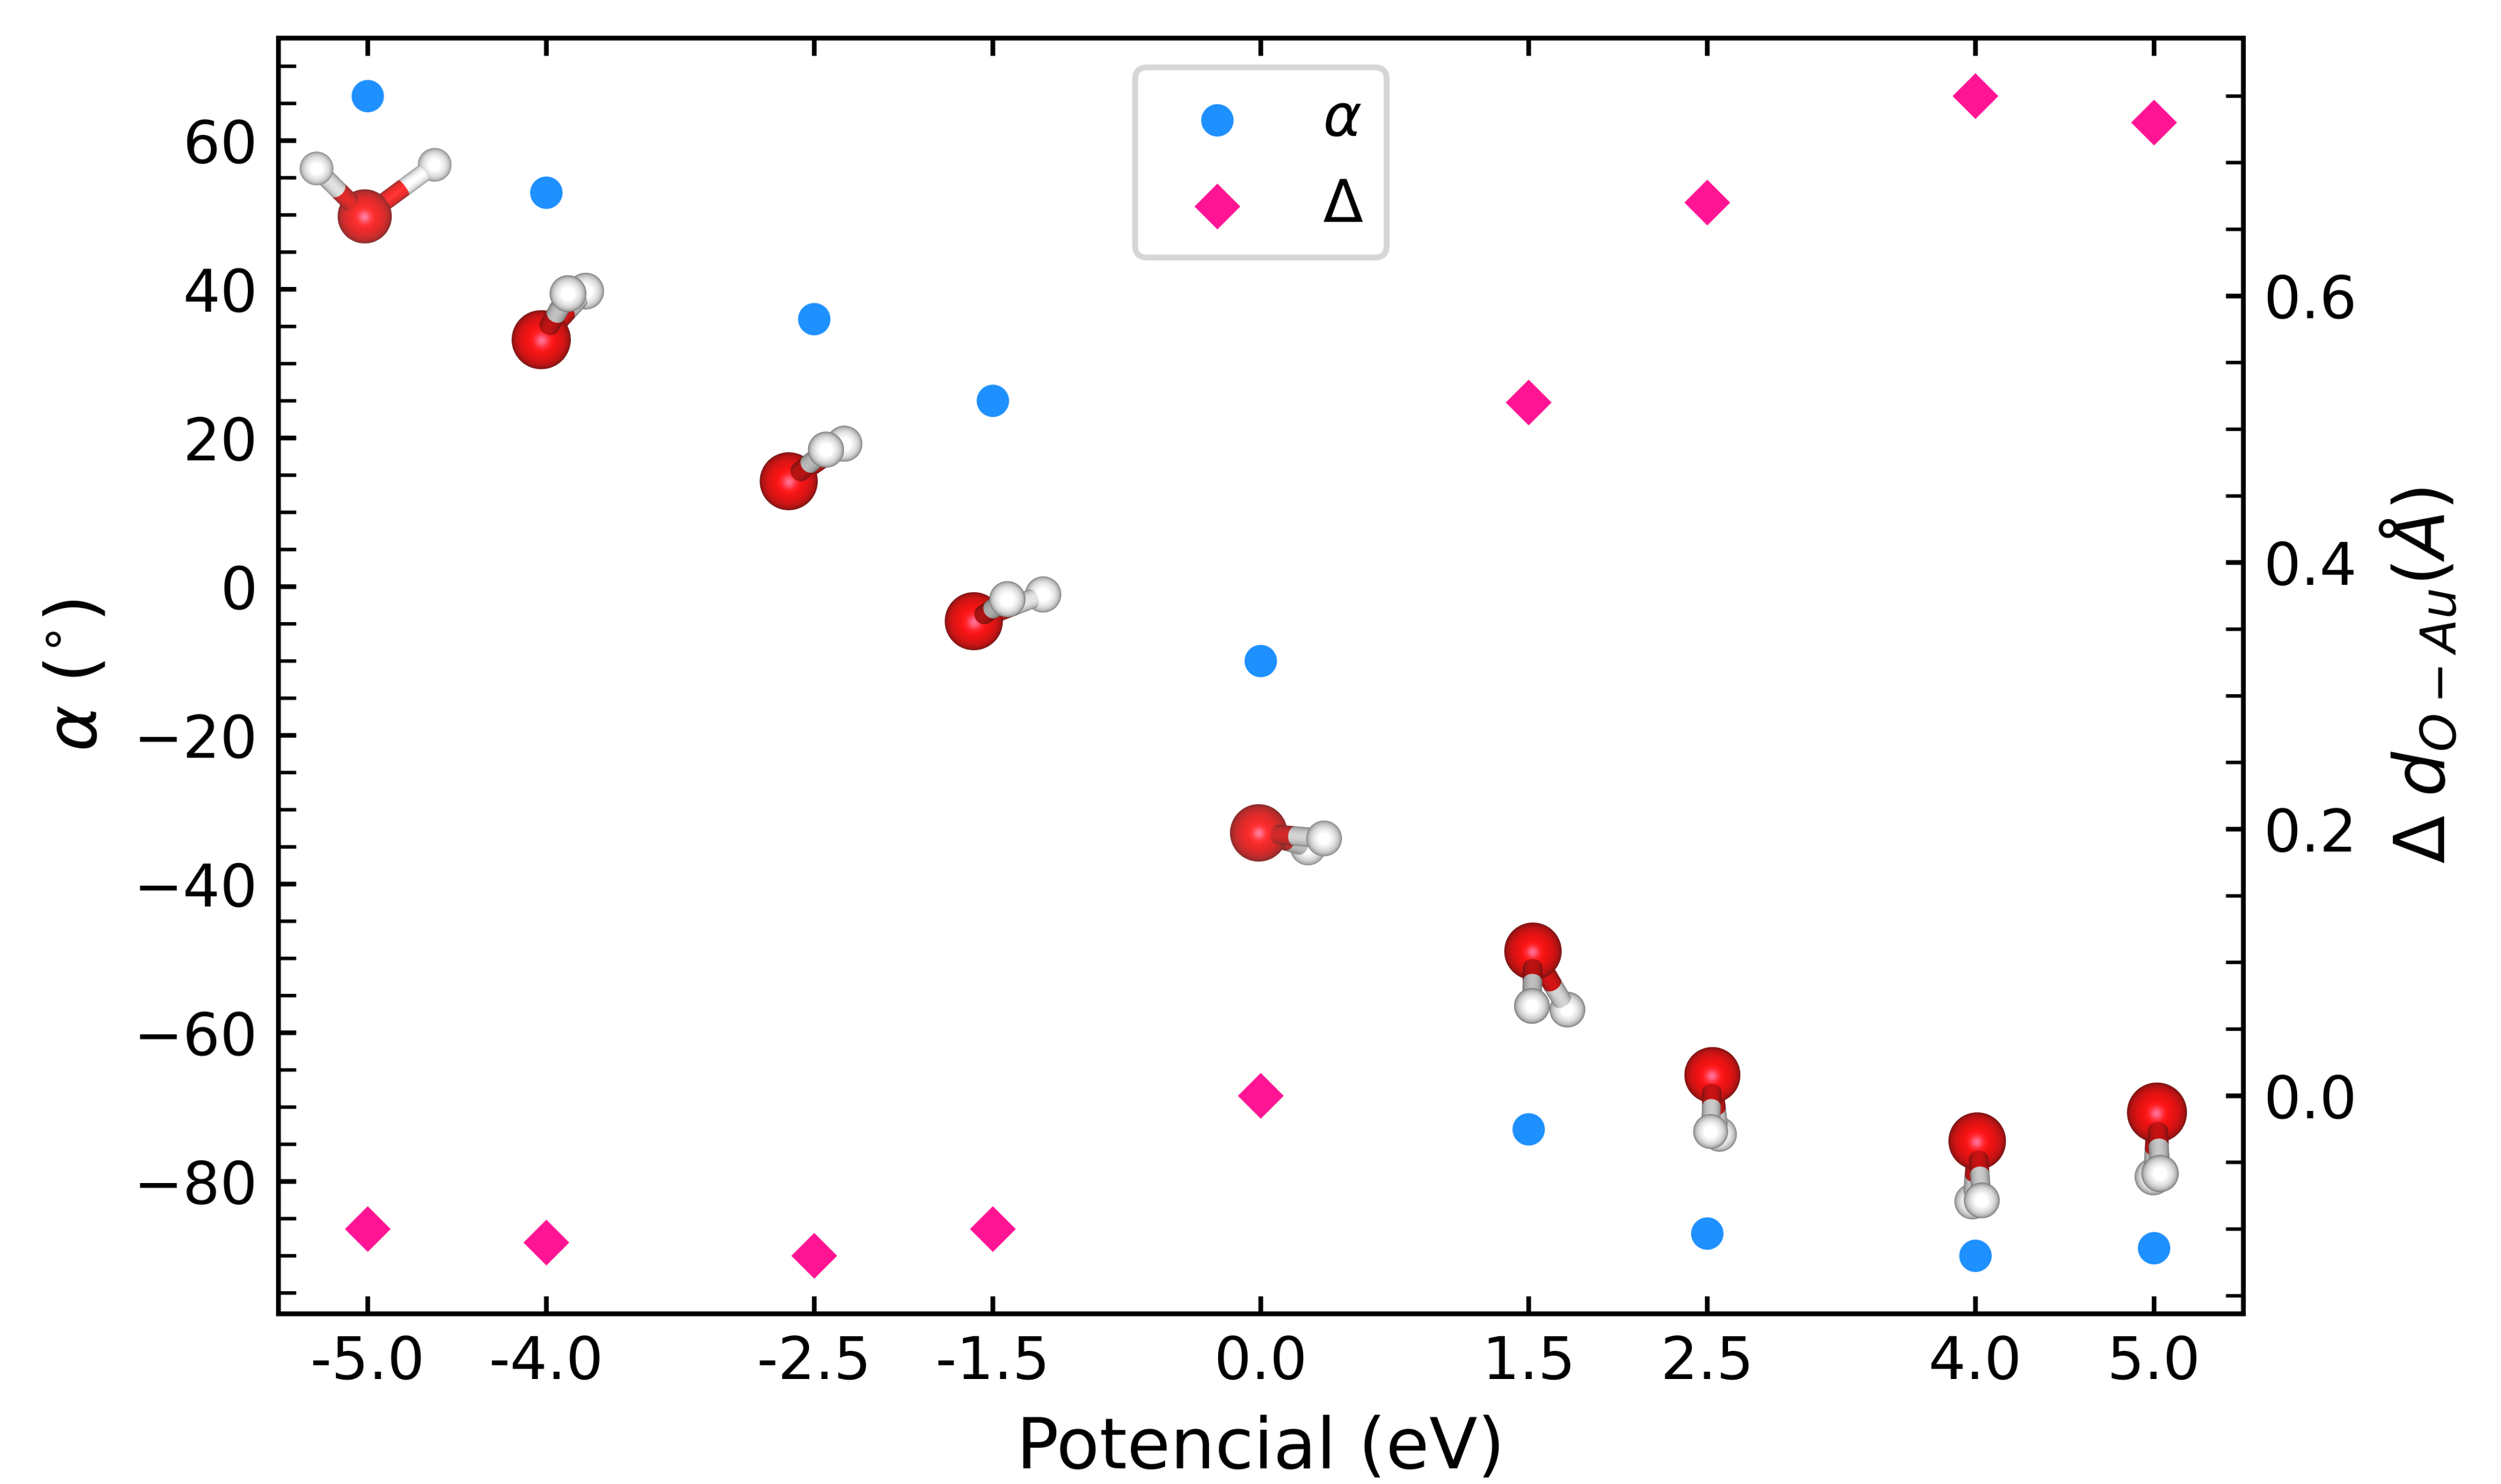
\includegraphics[scale=0.09]{figs/ang_monomer.jpg}
	\legend{Fonte: compilação da autora.}
\end{figure}

Ademais, observa-se que para $ V>2.5 \,\si{\eV} $, a inclinação da molécula $ \alpha $ praticamente não muda, ao passo que a variação da distância inicial muda progressivamente até 4.0 eV e depois apresenta um decréscimo. Esse efeito é resultado da polarização superficial do metal, no qual para potenciais positivos o átomo de oxigênio é repelido e os átomos de hidrogênio são atraídos; logo, a molécula fica na orientação \textit{down}. Para potenciais negativos observa-se o comportamento contrário, onde a variação da distância se mantém constante e com valor de $\Delta_{d_{O-Au}}= -0.1 \,\si{\angstrom} $ e as alterações ocorrem na inclinação em relação à superfície metálica; assim, a orientação da molécula se torna \textit{up}. De modo geral, percebe-se um comportamento padrão da molécula a partir de um determinado potencial: para potenciais positivos isso ocorre na inclinação e para os negativos na distância $ d_{O-Au} $.  

Como observado anteriormente, a aplicação do potencial altera também a reatividade do metal. No caso do Au, o potencial positivo intensifica o caráter hidrofóbico, fazendo com que a molécula se afaste mais do metal e também do sítio de adsorção \textit{atop}; isso é visto pelo aumento nas medidas $ d_{O-Au} $ e $ \Delta Oxy $. Em relação às propriedades intramoleculares, observa-se um alargamento do ângulo $ \Theta $ para os potenciais negativos e uma diminuição para os potenciais positivos. Assim como no Pd, as modificações estruturais são assimétricas e dependem do sinal do potencial aplicado. % Por outro lado, para o potencial negativo $ V=-1.5\,\si{\eV} $ a molécula se encontra acima do átomo de Au. 
 \begin{figure}[b!]
	\centering
	\caption{(a) Diferenças de densidades de carga $ \Delta \rho_{V} $ em relação ao potencial de 0.0 eV para os potenciais 1.5, 2.5 e 5.0 eV, cujos valores de isosuperfícies correspondem a $ 3.57\times10^{-4}\;\si{e}/\si{\angstrom}^3 $. Na última coluna estão representados as flutuações de densidades de carga com os respectivos valores de isosuperfícies $ 1.11\times10^{-5}$, $ 1.71\times10^{-5}$ e $ 5.57\times10^{-5}\;\si{e}/\si{\angstrom}^3 $. Em todos os casos, azul (vermelho) indica uma deficiência (excesso) de elétrons. (b) Gráfico das diferenças de densidades de carga média ao longo do eixo z de acordo com o potencial aplicado V.}
	\label{fig:neq_au_mon_dens}
	\includegraphics[scale=0.067]{figs/dens_bias-monomer.png}
	\legend{Fonte: compilação da autora.}
\end{figure}


O efeito de atração/repulsão da molécula de água pode ser visto por meio dos gráficos de diferença de densidade de carga $ \Delta\rho_V $ (Figura \ref{fig:neq_au_mon_dens} (a)). No gráfico, vemos uma maior concentração de carga no átomo de oxigênio e na superfície metálica. Essa concentração é proporcional ao aumento do potencial e possui um comportamento assimétrico entre o potencial positivo e negativo ($ \Sigma\Delta\rho_{_ {V}} $). Por meio do gráfico de flutuação média de carga ao longo do eixo z (Figura \ref{fig:neq_au_mon_dens} (b)), observa-se uma variação de densidade de carga na região da molécula e na última camada metálica; essas variações indicam transferência de carga entre a molécula e o metal. Portanto, a posição de equilíbrio do monômero para um dado valor de V é resultado da transferência de carga, interação eletrostática e repulsão de Pauli \cite{artigo-luana}.   

Após analisar como as interações e as propriedades estruturais são afetadas pelo potencial, investigamos os modos normais de vibrações da molécula de água (Tabela \ref{tab:neq_au_mon_freq}). Para a otimização realizada com PBC as frequências de \textit{bending} foi de $ 1642\,\si{\cm}^{-1} $ e as de \textit{stretching} simétrico e assimétrico foram $ 3644\,\si{\cm}^{-1}$ e $ 3758\,\si{\cm}^{-1} $, respectivamente. Comparando esses valores com os obtidos utilizando o formalismo de NEGF a V=0.0 eV, vemos que os valores são similares. Vale notar que as frequências de \textit{stretching} do monômero adsorvido no Au são superiores às frequências do Pd com o \textit{potencial 0}. Isso está relacionado ao fato da molécula estar mais afastada do Au em relação ao Pd e às propriedades de reatividade de cada superfície. 
 \begin{table}[t!]
	\centering
	\caption{Frequências dos modos normais de vibrações do monômero adsorvido no Au(111) de acordo com o potencial externo V aplicado.\label{tab:neq_au_mon_freq}}
	\begin{tabular}{Sccc} 
		\hline\hline\addlinespace[3.6pt]
		\multicolumn{4}{c}{\textbf{Frequências dos Modos Normais $ H_2O/Au\,(\mathbf{\si{\cm}^{-1}})$}}\\ \midrule
		{V (eV)}   &$Bending$	&$\textit{Stretching} \, (S)$	&$\textit{Stretching} \, (AS)$\\
		\hline
		5.0		&1642	&3597	&3687\\
		4.0		&1639	&3613	&3685\\	
		2.5		&1630	&3618	&3704\\	
		1.5		&1623	&3602	&3697\\
		0.0		&1626	&3646	&3759\\
		-1.5		&1624	&3675	&3790\\
		-2.5		&1630	&3671	&3798\\
		-4.0		&1638	&3673	&3797\\
		-5.0		&1647	&3653	&3789\\ %\midrule
	%	PBC		&1624	&3644	&3758 \\
		\hline\hline
	\end{tabular}
	\legend{Fonte: compilação da autora.}
\end{table}


\begin{figure}[h!]
	\centering
	\caption{Distribuições das densidades de estados vibracionais (unidades arbitrárias) de acordo com potencial externo aplicado na interface monômero/Au. As distribuições estão divididas de acordo com os modos fundamentais do monômero \textit{bending}, \textit{stretching} e translacionais. As linhas tracejadas representam os valores experimentais do monômero isolado.}
	\label{fig:neq_au_mon_freq}
	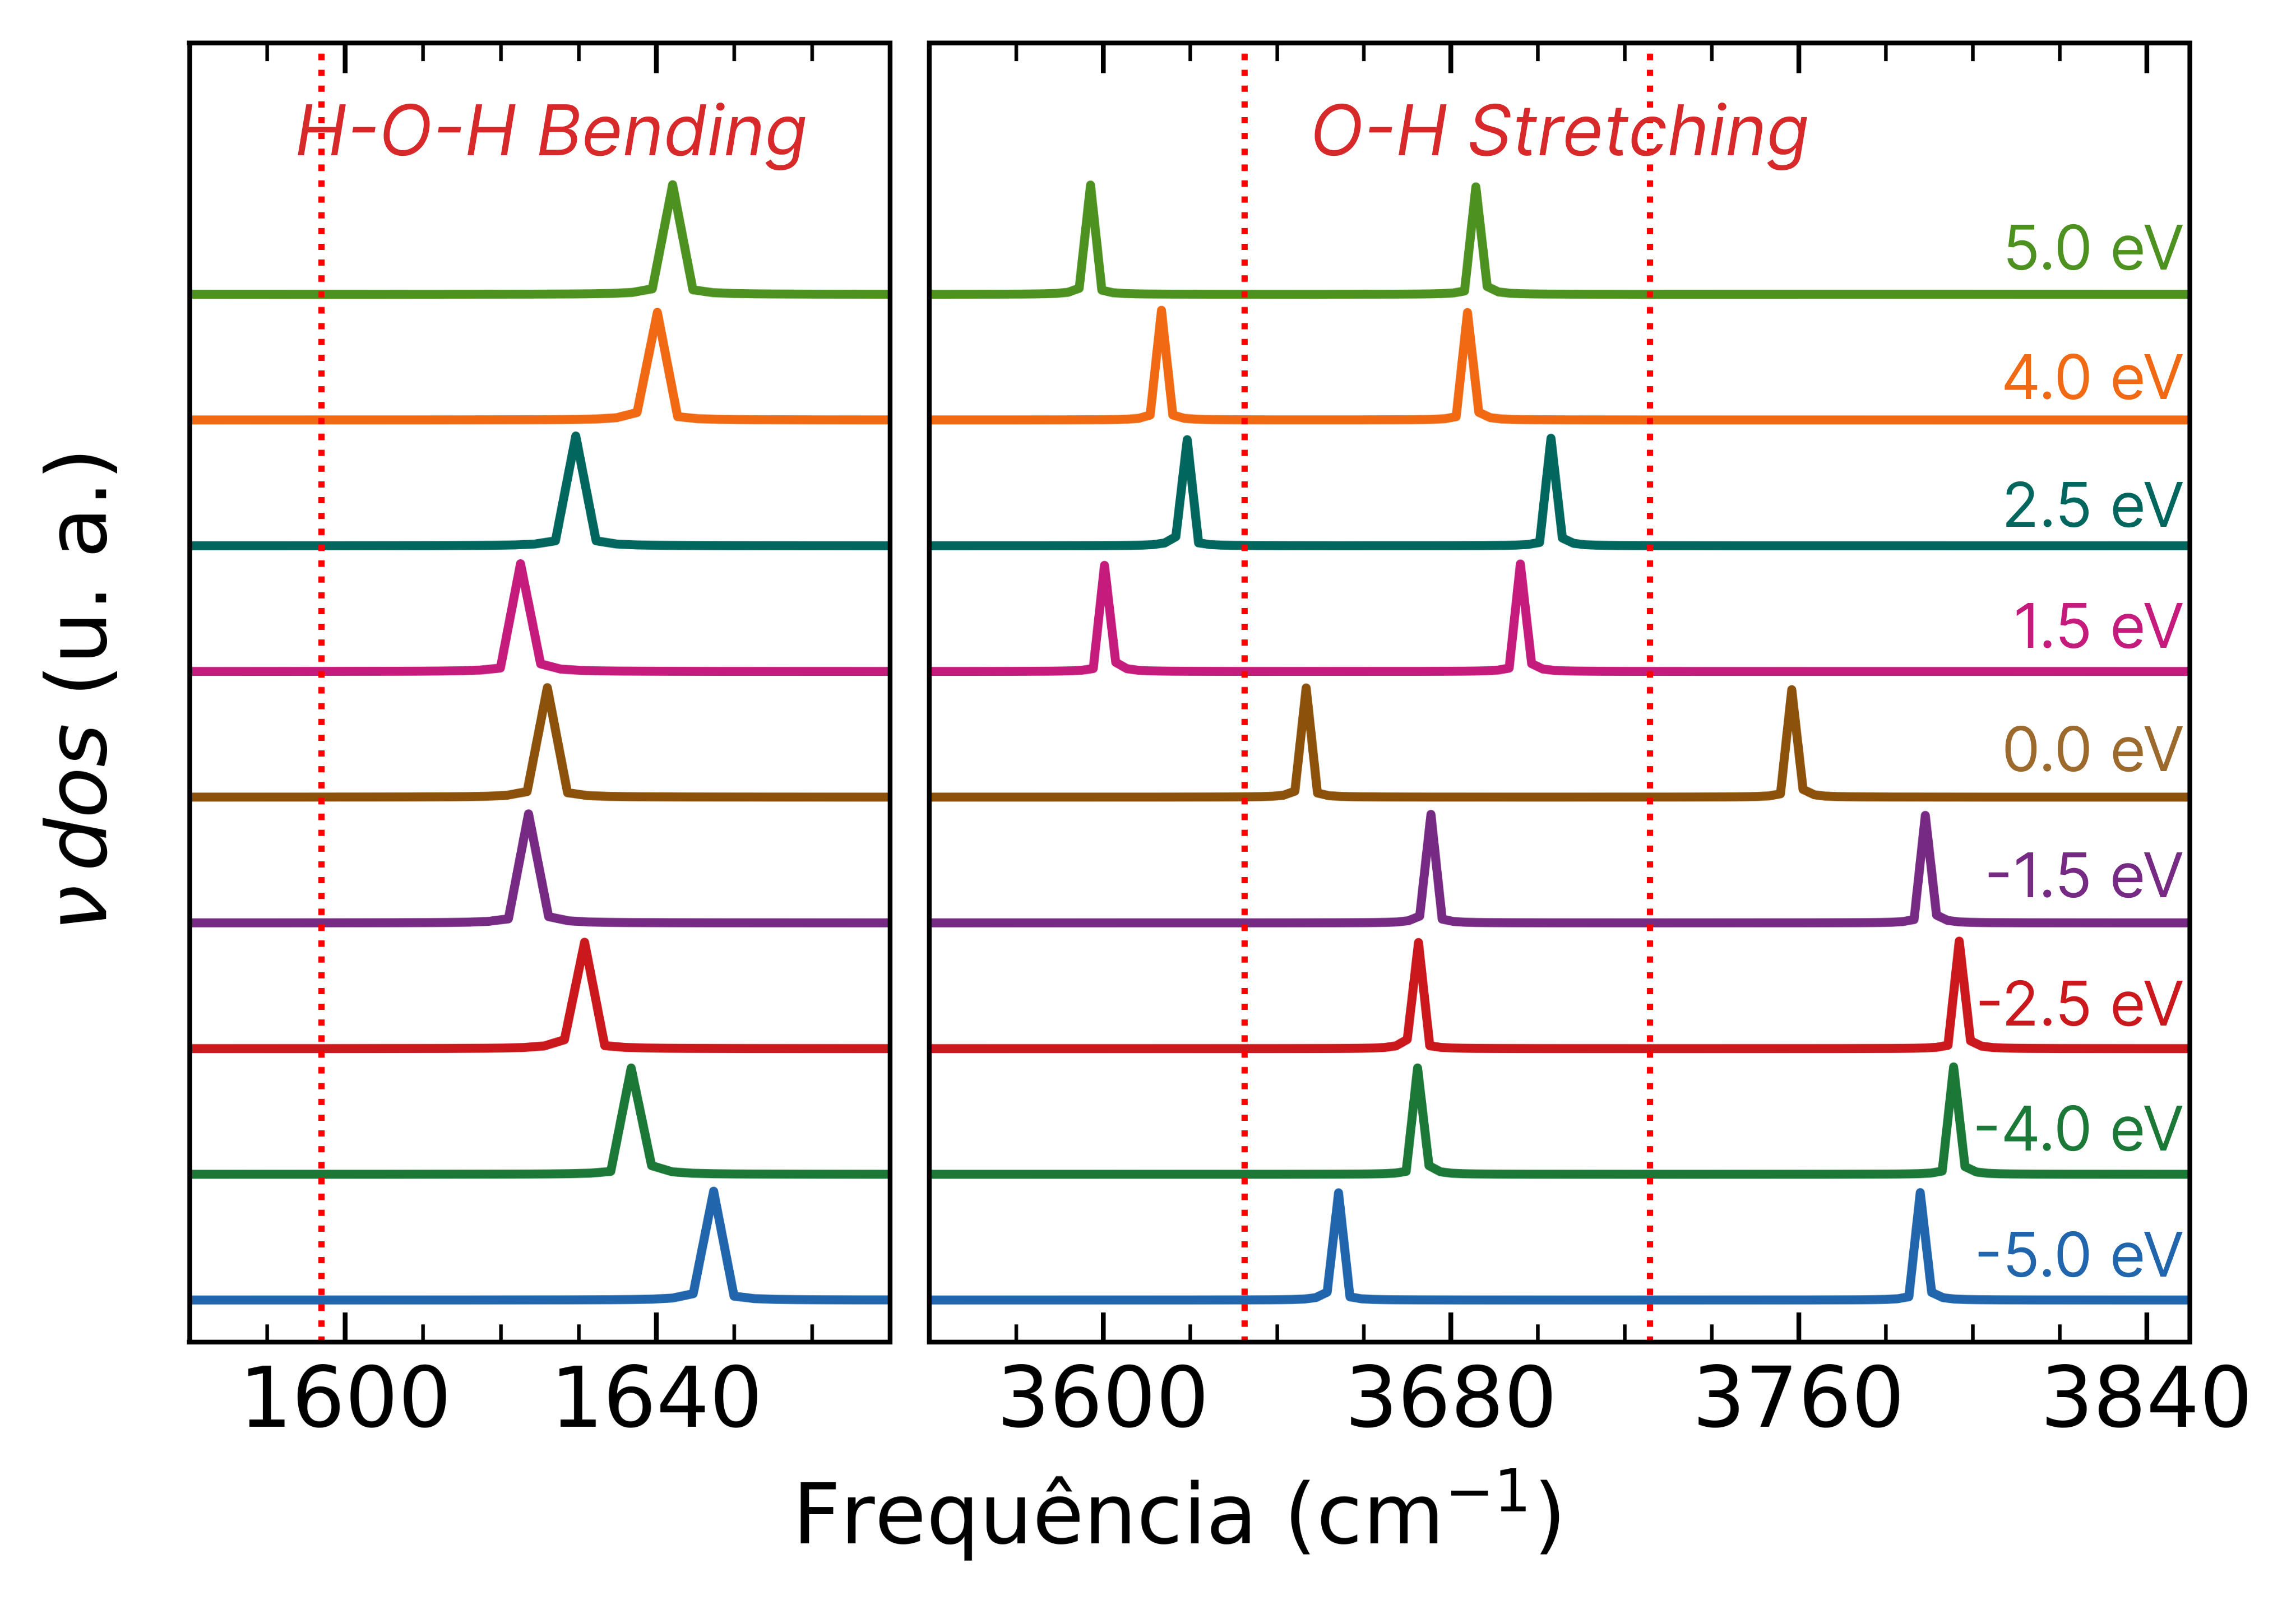
\includegraphics[scale=0.08]{figs/freq_monomer_au.png}
	\legend{Fonte: compilação da autora.}
\end{figure}


Para os potenciais negativos observa-se que a frequências de \textit{stretching} antissimétrico aumenta $ 31\,\si{\cm}^{-1} $ e depois se mantém praticamente constante; por outro lado, para a frequência de \textit{stretching} simétrico, observa-se um aumento de $ 29\,\si{\cm}^{-1} $ e em seguida uma redução nas frequências. Esse aumento das frequências está associado a menor interação das ligações O-H com o metal devido à rotação das moléculas na direção contrária à superfície. Para V>0, observa-se uma tendência de redução nas frequências de \textit{stretching} por causa da maior proximidade das ligações O-H com o metal,no qual a redução máxima do \textit{stretching} simétrico foi de $ 49\,\si{\cm}^{-1} $ e do assimétrico $ 74\,\si{\cm}^{-1} $. 

Com o intuito de investigar se a aplicação do potencial sobre o monômero era reversível e identificar possíveis transições de fases, foi realizado a otimização da estrutura através de  voltametria cíclica -- Figura \ref{fig:neq_au_voltametria} (c). Nas otimizações descritas anteriormente, as coordenadas iniciais das relaxações eram as obtidas a partir da relaxação do \textit{potencial 0}. No processo de voltametria, utilizava-se as coordenadas finais da relaxação a V=5.0 eV para realizar a otimização a $ V=4.0\,\si{\eV}$; isso era feito progressivamente até atingir $ V=5.0\,\si{\eV}$ (sentido negativo). O mesmo foi feito para $ V=-5.0\,\si{\eV}$ até atingir $ V=5.0\,\si{\eV}$ (sentido positivo). Em seguida, para cada otimização era calculado os modos normais de vibrações, onde as frequências de \textit{stretching} estão representadas na Figura \ref{fig:neq_au_voltametria} (a) e (b). 

%\todo[inline,color=green!40]{Falar um pouco mais sobre os resultados experimentais.}

Assim, o que se observa é que para as frequências de \textit{stretching} simétrico e assimétricos, as curvas do sentido positivo e negativo seguem a mesma tendência e apresentam variações dentro da margem de erro. Portanto, os diferentes processos pelos quais se aplica a variação do potencial são equivalentes. Por outro lado, experimentalmente observa-se processos de oxidação e redução na superfície metálica ao realizar a voltametria cíclica que são observados a partir das alterações nas frequências vibracionais \cite{sfg_kramer}. De acordo com \citeauthor{sfg_kramer}, esses processos estão relacionados ao efeito da superfície carregada sobre as moléculas de água e também devido às interações entre as moléculas da interface com as moléculas da água \textit{bulk}. 

\begin{figure}[h!]
	\centering
	\caption{(a) Frequências de \textit{Stretching} simétrico e (b) assimétrico do monômero adsorvido no Au(111) obtidas na voltametria cíclica, respectivamente. (c) Esquema da aplicação do potencial externo sobre o sistema na voltametria cíclica.}
	\label{fig:neq_au_voltametria}
	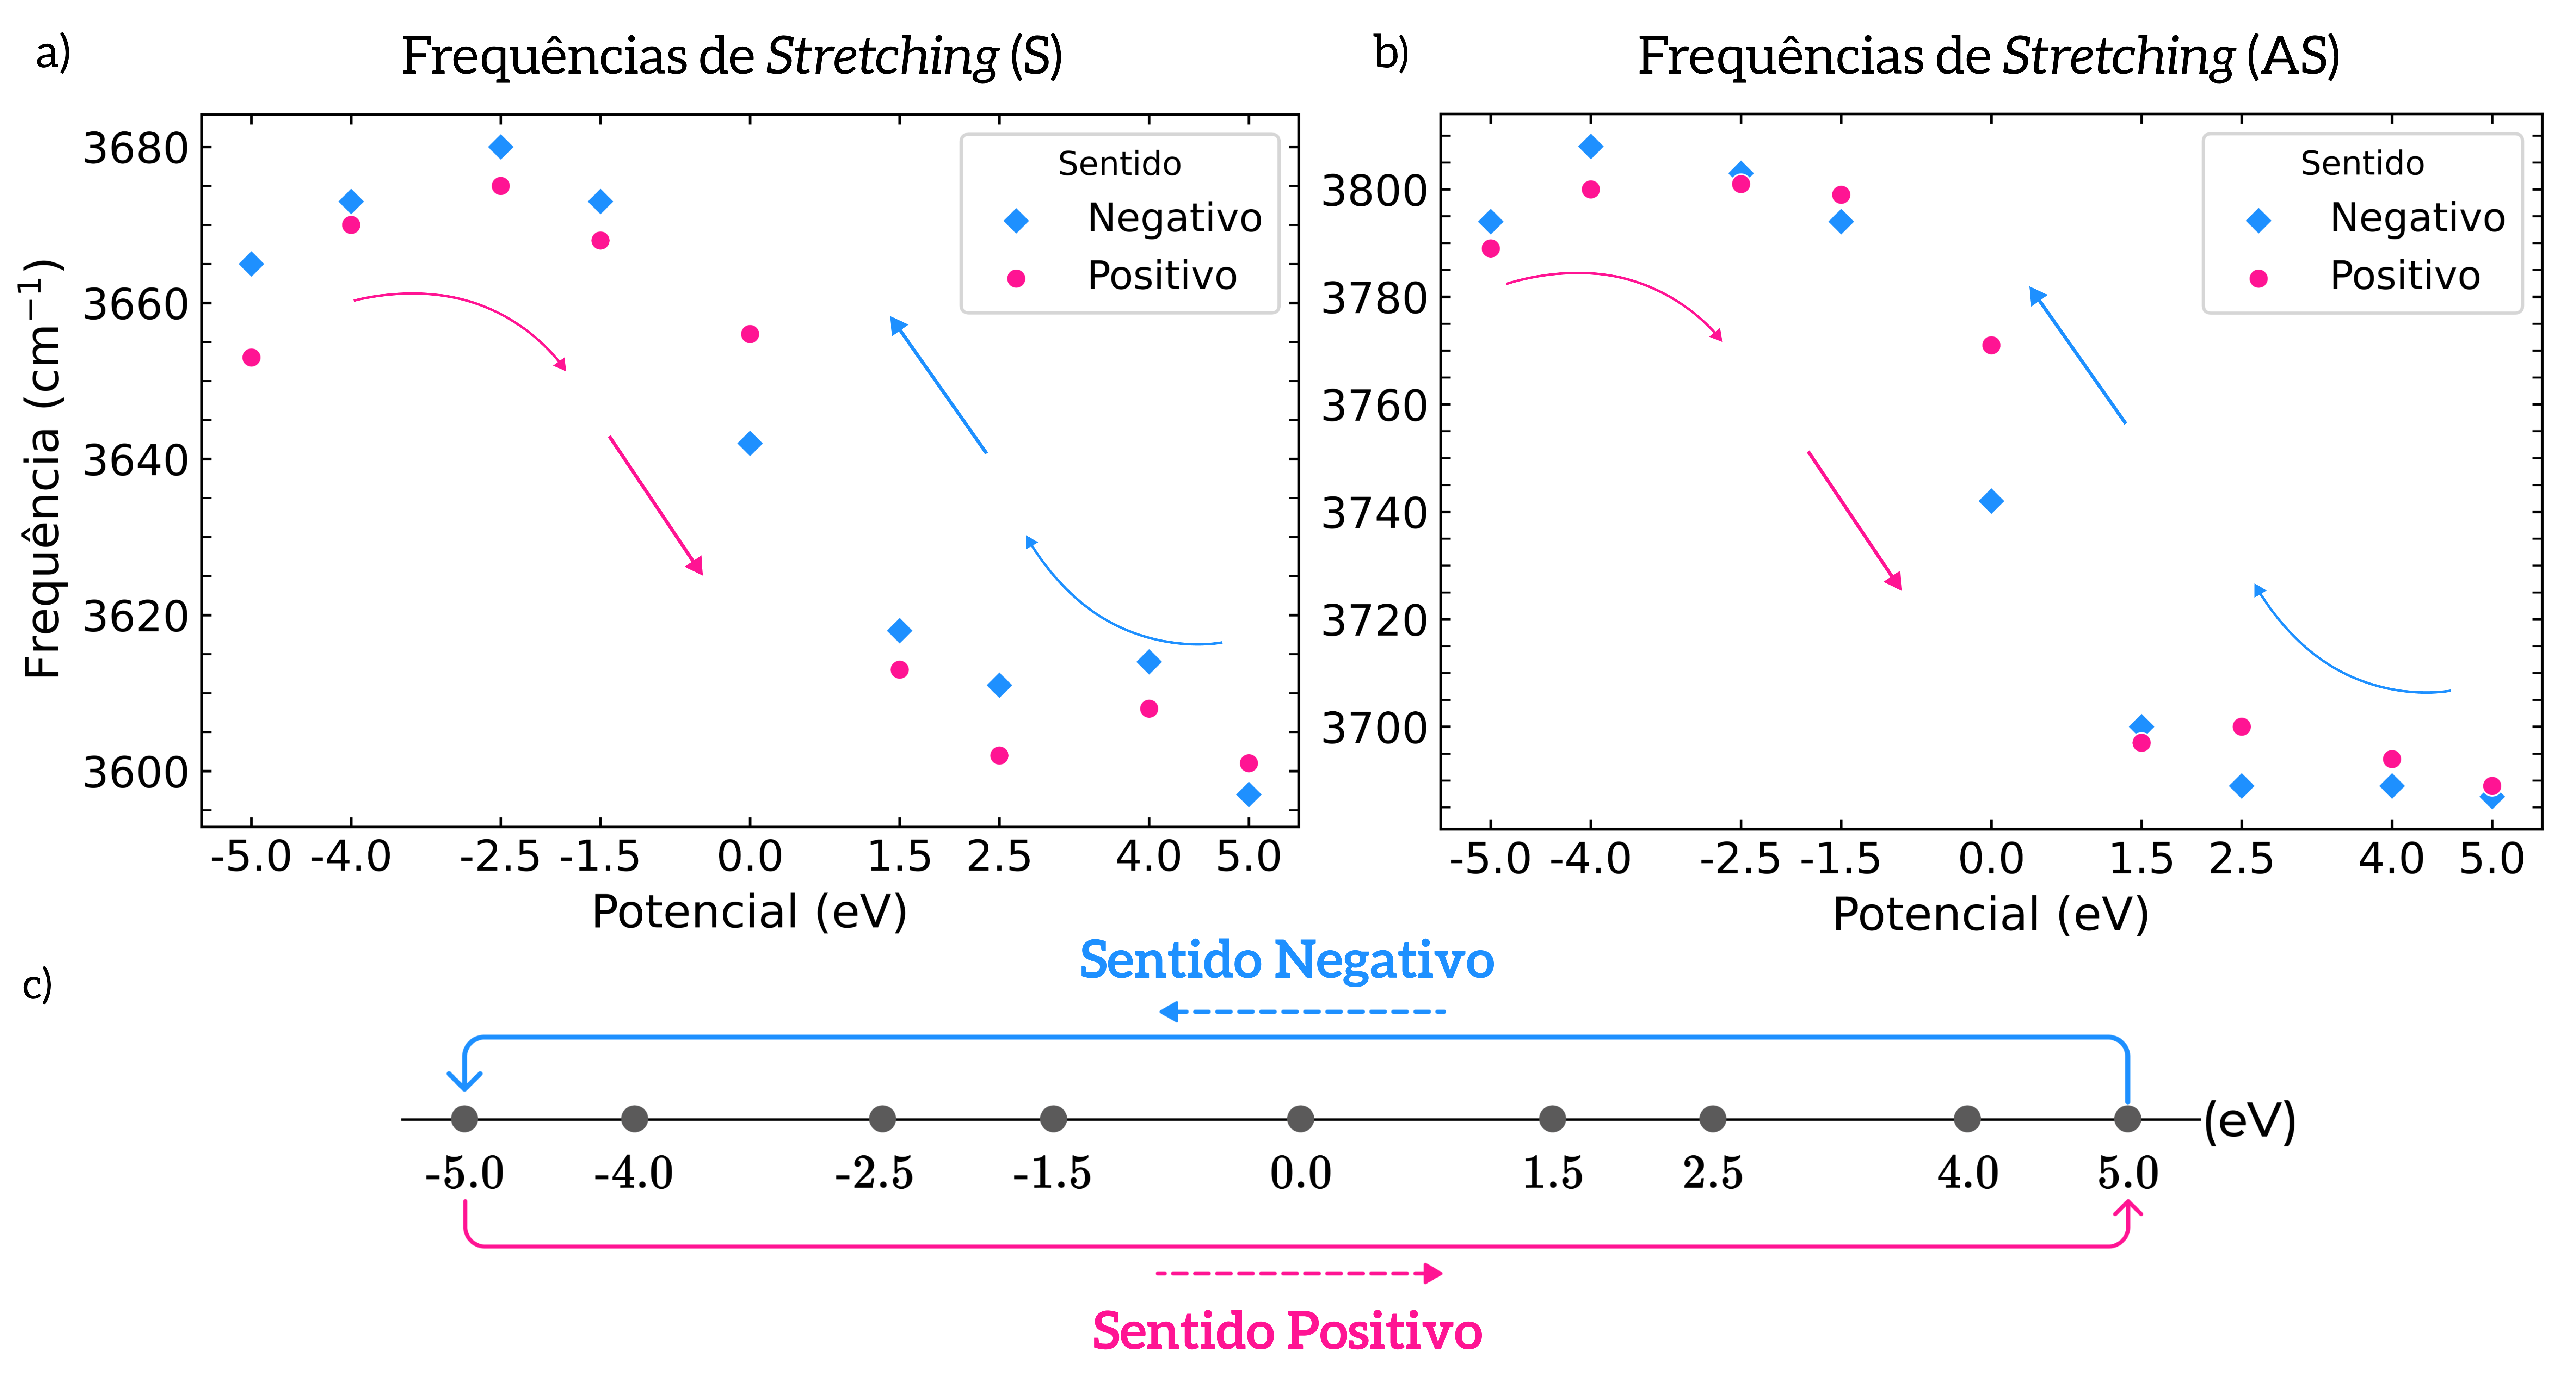
\includegraphics[scale=0.06]{figs/voltametria_monomer.png}
	\legend{Fonte: compilação da autora.}
\end{figure}

\subsection{Camada de Água \label{sec:neq_au_layer}}

Após caracterizar a interação água/metal sob a influência do potencial externo, investigamos como as ligações de hidrogênio são afetadas. Para isso, aplicamos um potencial externo sobre uma camada do tipo \textit{H-Down} adsorvida numa superfície metálica de Au(111) (Figura \ref{fig:neq_au_geo_layer}). Essa camada foi escolhida, pois resultados teóricos utilizando cálculos de DFT a mostraram como mais estável \cite{monomer}. 

No entanto, no âmbito experimental, a orientação exata da molécula de água na interface com o metal ainda é indefinida, principalmente considerando um potencial externo sobre o sistema. Nesse sentido, no estudo experimental conduzido por \citeauthor{sfg_kramer} foi observado alterações vibracionais ao aplicar uma variação de potencial na interface água/Au (111), as quais foram associadas às modificações estruturais. De acordo com os autores, os resultados indicam ligações O-H apontando para o metal (\textit{dangling OH-bonds}) no potencial de carga zero, de forma que, ao aplicar a diferença de potencial essas ligações são atraídas para a superfície metálica quando o potencial é negativo ou repelidas para potenciais positivos. Esse comportamento também foi observado em simulações computacionais, onde \citeauthor{pd_bias_layer} examinaram a adsorção de uma camada de água no Pd(111) e encontraram transição de fase de primeira ordem a partir de um determinado potencial através do cálculo da energia livre. Os autores associaram essa transição à mudança de orientação das moléculas de \textit{flat-down} para \textit{flat-up}.
\begin{table}[b!]
	\centering
	\caption{Propriedades geométricas médias da Camada de água adsorvida no Au (111) de acordo com o potencial externo V aplicado. As distâncias analisadas foram tomadas em relação aos valores médios das moléculas nas orientações \textit{flat-down} e \textit{flat} e correspondem a: distâncias entre os átomos de O ($ {d_{OO}} $), distâncias entre os átomos de O e Au ${d_{O-Au}}(\si{\angstrom})$, inclinação $ \alpha $ em relação à superfície, distância entre os átomos de H e O $ {d_{O-H}}(\si{\angstrom})$, onde o primeiro valor corresponde à ligação OH com o metal e segundo à ligação de hidrogênio, além do ângulo médio $ \Theta $ entre os átomos de H.}
	\begin{tabular}{Scccccccccc} 
		\hline\hline\addlinespace[3.5pt]
		\multicolumn{11}{c}{\textbf{Propriedades Geométricas ($ \si{\angstrom} $) -- Camada de Água/Au(111)}}  \\                                                                                                 
		\midrule
		{\multirow{2}{*}{{V(eV)}}}                                                                                                    & \multicolumn{2}{c}{${d_{OO}}$} & \multicolumn{2}{c}{\textbf{${d_{O-Au}}$}} &  \multicolumn{2}{c}{$\alpha$}& \multicolumn{2}{c}{\textbf{${d_{O-H}}$}}& \multicolumn{2}{c}{$\Theta$} \\ 
		\cmidrule{2-11}      &$ {d_{OO1}} $ &$ {d_{OO2}} $                  & \textit{Down}  & \textit{Flat}	&\textit{Down}  &\textit{Flat}	&\textit{Down}  &\textit{Flat}  &\textit{Down}  &\textit{Flat}   \\
		\midrule
		-5.00 & 2.97&3.02 &3.31  &2.93&-39  &28 	 &$0.98\,/ \, 0.99$  &$0.98$&102  &105     \\
		-4.00 &2.96&3.03 & 3.31  &2.96	 &-40  &26   &$0.98\,/ \, 0.99$  &$0.98$	&  102  &105    \\
		-2.50 &3.93&3.04 & 3.32  &3.03 &-41  &24  	 &$0.98\,/ \, 0.99$  &$0.98$	&  102  &105      \\
		-1.50 &2.92&3.04 & 3.33  &3.09	 &  -42  &21  &$0.98\,/ \, 0.99$  &$0.98$	&  102  &105     \\
		0.00 &2.90&3.05 & 3.35  &3.18	&  -42  &18  &$0.98\,/ \, 0.99$  &$0.98$	&  102  &106     \\
		1.50 &2.89&3.05 & 3.37  &3.29&  -43  &14 	  &$0.98\,/ \, 0.99$  &$0.98$	&  102  &106     \\
		2.50 &2.88&3.06 & 3.37  &3.35  &-43  &10	&  $0.98\,/ \, 0.99$  &$0.98$	&  102  &106     \\
		4.00 &2.88&3.07 & 3.41  &3.58&-42  &0  	&  $0.98\,/ \, 0.99$  &$0.98$	&  102  &106      \\
		5.00 &2.88&3.09 & 3.44  &3.75	&  -41  &-7   &$0.98\,/ \, 0.99$  &$0.98$	&  103  &106    \\ \midrule
	%	PBC && & 3.34  &3.13	&  0.98  &0.98	&  102  &105   &-42  &19   \\
		\hline\hline 
	\end{tabular}
	\legend{Fonte: compilação da autora.}
\end{table}

\begin{figure}[h!]
	\centering
	\caption{(a)Variação média da inclinação $ \alpha $ e da distância inicial $ \Delta d_{O-Au} $ das moléculas \textit{flat} de acordo com o potencial. A variação da distância $ \Delta d_{O-Au}= d_{O-Au,V}-d_{0}$ foi determinada em relação à posição inicial média $ d_0=3.18\,\si{\angstrom}$ obtida após a relaxação com o \textit{potencial 0}. Abaixo, a posição das moléculas \textit{flat-down} e \textit{flat} foi ilustrada para diversos potenciais e ao lado está representado as medidas representadas no gráfico. (b) Variações das distâncias médias $ d_{OO1} $ e $ d_{OO2} $ entre os átomos de O de acordo com o potencial aplicado.}
	\begin{subfigure}{0.9\textwidth}            
		\caption{\textit{Variações de $ \alpha $ e $ \Delta d_{O-Au} $das moléculas \textit{flat}}.}
		\centering
		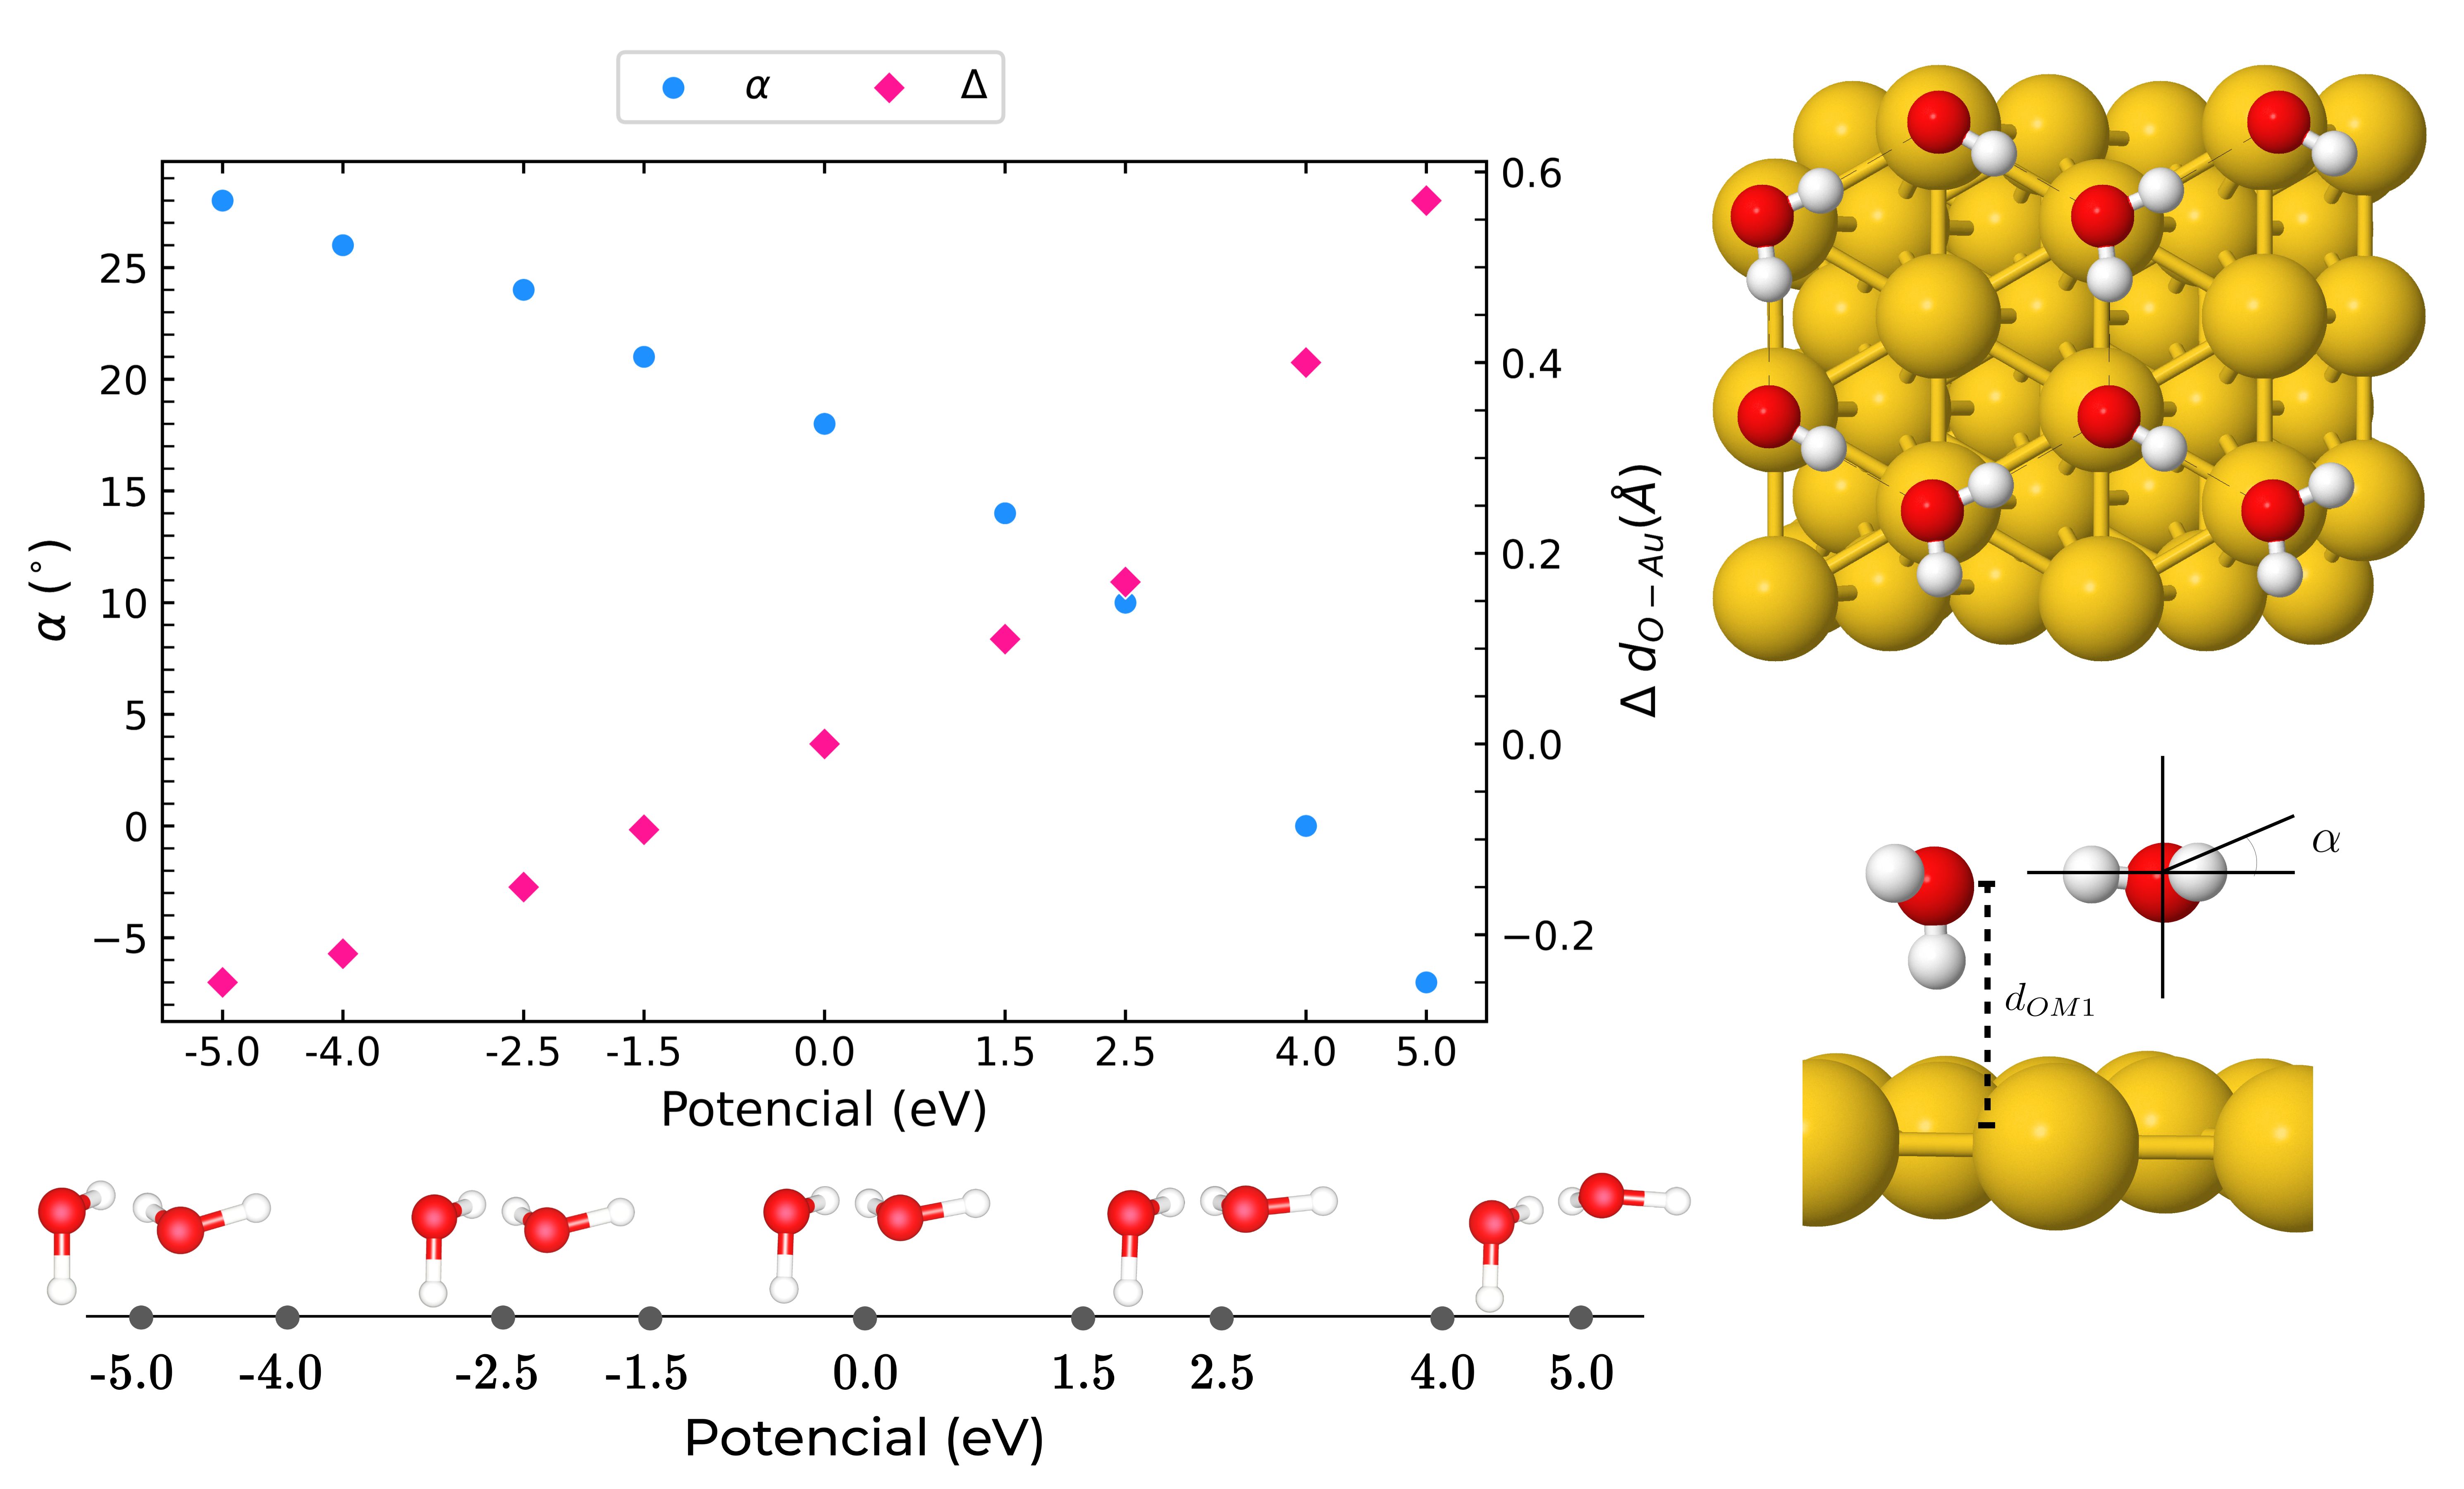
\includegraphics[width=\textwidth]{figs/ang_layer.png}
		\legend{Fonte: compilação da autora.}
		\label{fig:neq_au_geo_layer}
	\end{subfigure}\,
	\begin{subfigure}{0.7\textwidth}
		\caption{\textit{Variações das distâncias $ d_{O-O} $.}}
		\centering
		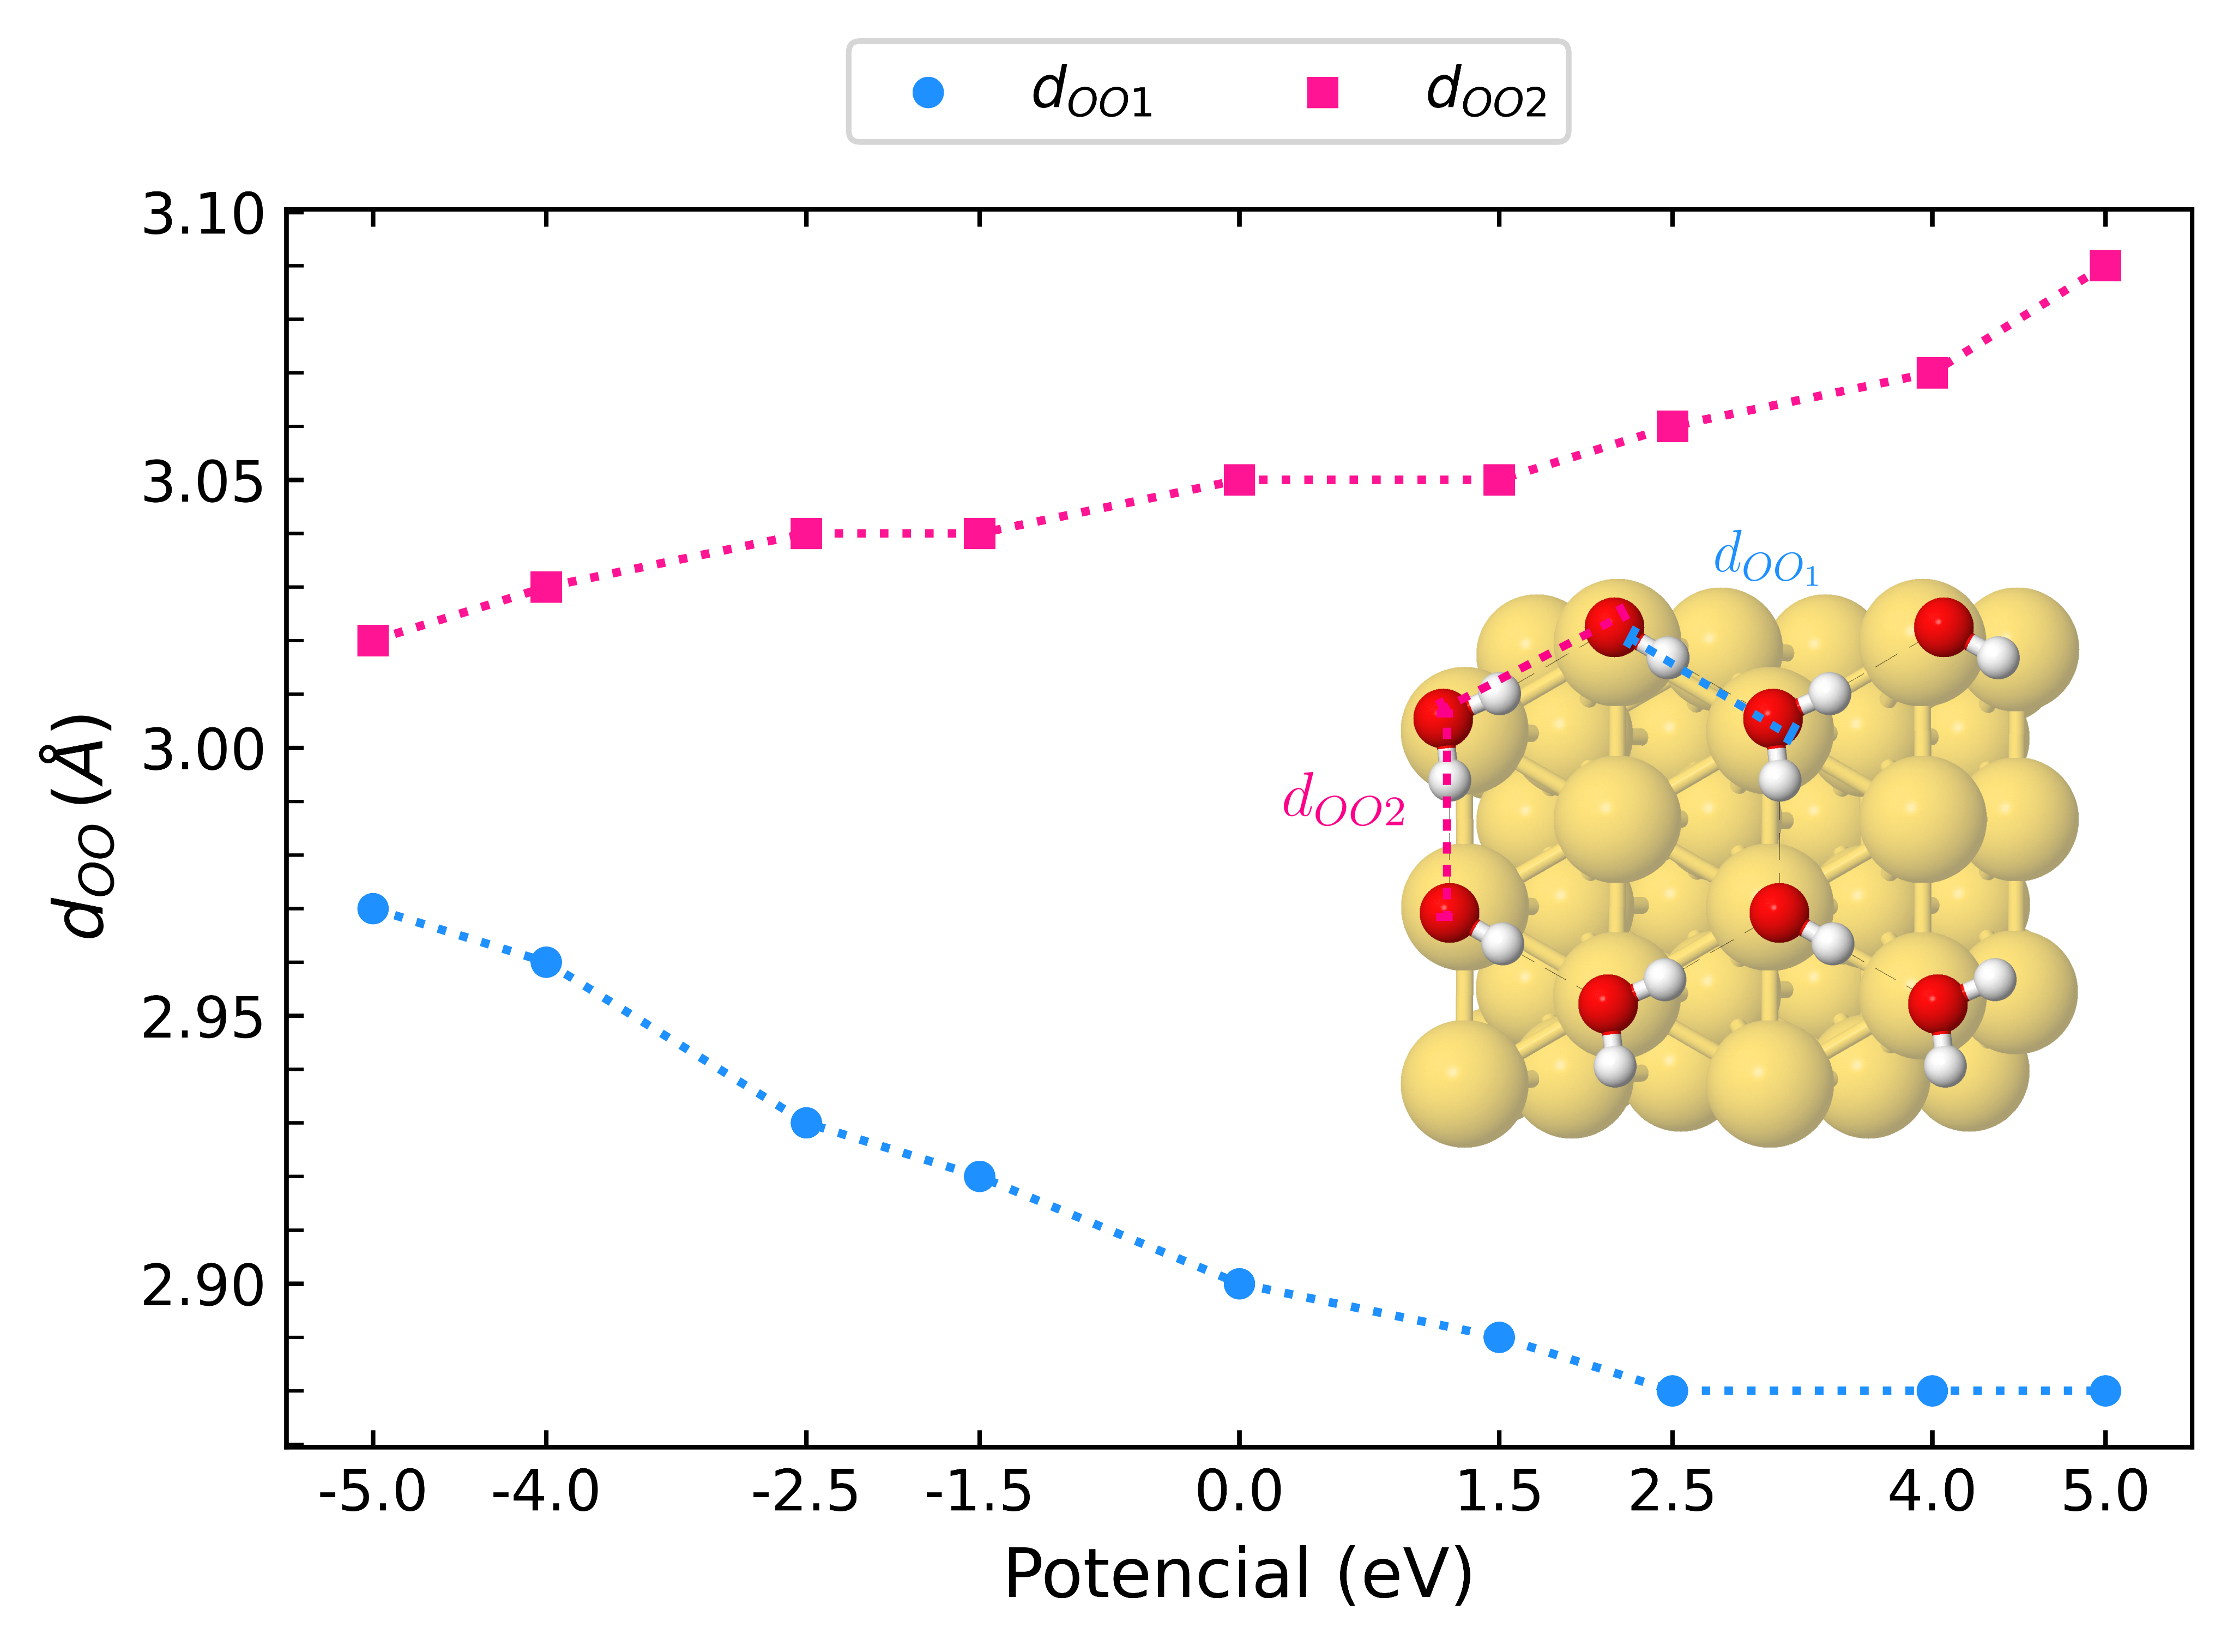
\includegraphics[width=\textwidth]{figs/distancia_oo.png}
		\legend{Fonte: compilação da autora.}
		\label{fig:distancia_oo}
	\end{subfigure}
\end{figure}

Dessa forma, a camada de água estudada nesse trabalho possuía 8 moléculas dispostas num arranjo hexagonal semelhante ao do gelo (\textit{ice bilayer Ih}) em uma célula de tamanho $ (\sqrt{3}\times\sqrt{3})R30 $ em relação ao parâmetro estrutural do Au ($ 4.24\,\si{\angstrom} $). Os eletrodos metálicos eram compostos por 3 camadas com o plano metálico formado por $ 3\times 4$ átomos nas direções $ xy $. O tamanho da célula unitária utilizada foi $ 10.40\times9.00\times 54.21\,\si{\angstrom} $. O funcional de troca e correlação utilizado foi o PBE e as relaxações foram realizadas com os potencias externo variando entre -5.0 a 5.0 eV, com intervalos entre 1.0 a 1.5 eV. Após obter as coordenadas minimizadas, obteve-se as frequências de vibrações do sistema.

Em relação às moléculas na orientação \textit{flat-down}, observa-se variações máximas de $\Delta_{d,máx}= 0.09\,\si{\angstrom} $ e da inclinação $\Delta_{\alpha,máx}= 3\si{\degree} $, ao passo que as variações máximas das moléculas \textit{flat} foram $\Delta_{d,máx}= 0.57\,\si{\angstrom} $ e $\Delta_{\alpha,máx}= 25\si{\degree} $, respectivamente (Tabela \ref{tab:neq_au_geo}). Para potenciais positivos, as moléculas tendem a se afastar da superfície metálica, enquanto que para potenciais negativos as moléculas se aproximam do metal. Além disso, é possível ver o efeito da competição entre a interação água/metal e a ligação de hidrogênio, uma vez que, as variações das distâncias e das inclinações são menores que as observadas no monômero. Esse efeito também é visto pelo aumento da ligação $ d_{O-H} $ em relação ao monômero $ d_{O-H}\sim0.97\,\si{\angstrom} $; para as moléculas \textit{flat-down} a distância $ d_{O-H} $ da ligação O-H que interage com o metal foi $ 0.98\,\si{\angstrom}  $, ao passo que a ligação O-H que participa da ligação de hidrogênio foi $ 0.99\,\si{\angstrom}  $. Esses valores são inferiores aos observados na camada de água \textit{H-Down} adsorvida no Pd(111), onde obtivemos $ d_{OH}=0.99\,\si{\angstrom} $ para a ligação O-H que participa da ligação de hidrogênio e $ d_{OH}=1.00\,\si{\angstrom} $ para a ligação que interage com o metal. Esse resultado revela o efeito das propriedades reativas do metal sobre a adsorção de estruturas de água.

O efeito do potencial externo afeta principalmente as moléculas \textit{flat}, uma vez que as propriedades geométricas das moléculas \textit{flat-down} apresentaram alterações pequenas com a variação do potencial. Ademais, observa-se que os ângulos $ \Theta $ das moléculas \textit{flat} são maiores do que os da molécula \textit{flat-down}. Além disso, é possível ver o comportamento assimétrico das propriedades geométricas em relação ao sinal do potencial aplicado. Isso é visto através da inclinação $ \alpha $ que somente troca de sinal a partir de V=2.5 eV, diferentemente do caso do monômero. Além disso, observa-se que as moléculas se afastam do metal e diminuem a inclinação para potenciais positivos e se aproximam e aumentam a inclinação para V<0. Esses processos ocorrem de forma quase linear e refletem atração/repulsão resultante da polarização superficial e o aumento/diminuição da repulsão de Pauli.

\begin{figure}[t!]
	\centering
	\caption{(a) Diferenças de densidades de carga $ \Delta \rho_{V} $ da camada de água adsorvida no Au(111) para os potenciais 1.5 e 5.0 eV. Os valores de isosuperfícies dos gráficos de $ \Delta\rho_{+V} $ e $ \Delta\rho_{-V} $ correspondem a $ 3.97\times10^{-4}\;\si{e}/\si{\angstrom}^3 $. Na última coluna estão representados as flutuações de densidades de carga com os respectivos valores de isosuperfícies $ 3.35\times10^{-5}$ e $ 1.60\times10^{-5}$. Em todos os casos, azul (vermelho) indica uma deficiência (excesso) de elétrons. (b) Gráfico das diferenças de densidades de carga média ao longo do eixo z para os potenciais $ V=\pm1.5\,\pm2.5$ e $ \pm5.0\,\si{\eV} $. No gráfico também estão representados as posições da última camada de Au, dos átomos de H das moléculas \textit{flat-down} que interagem com o metal e dos átomos de oxigênio das moléculas \textit{flat-down}.}
	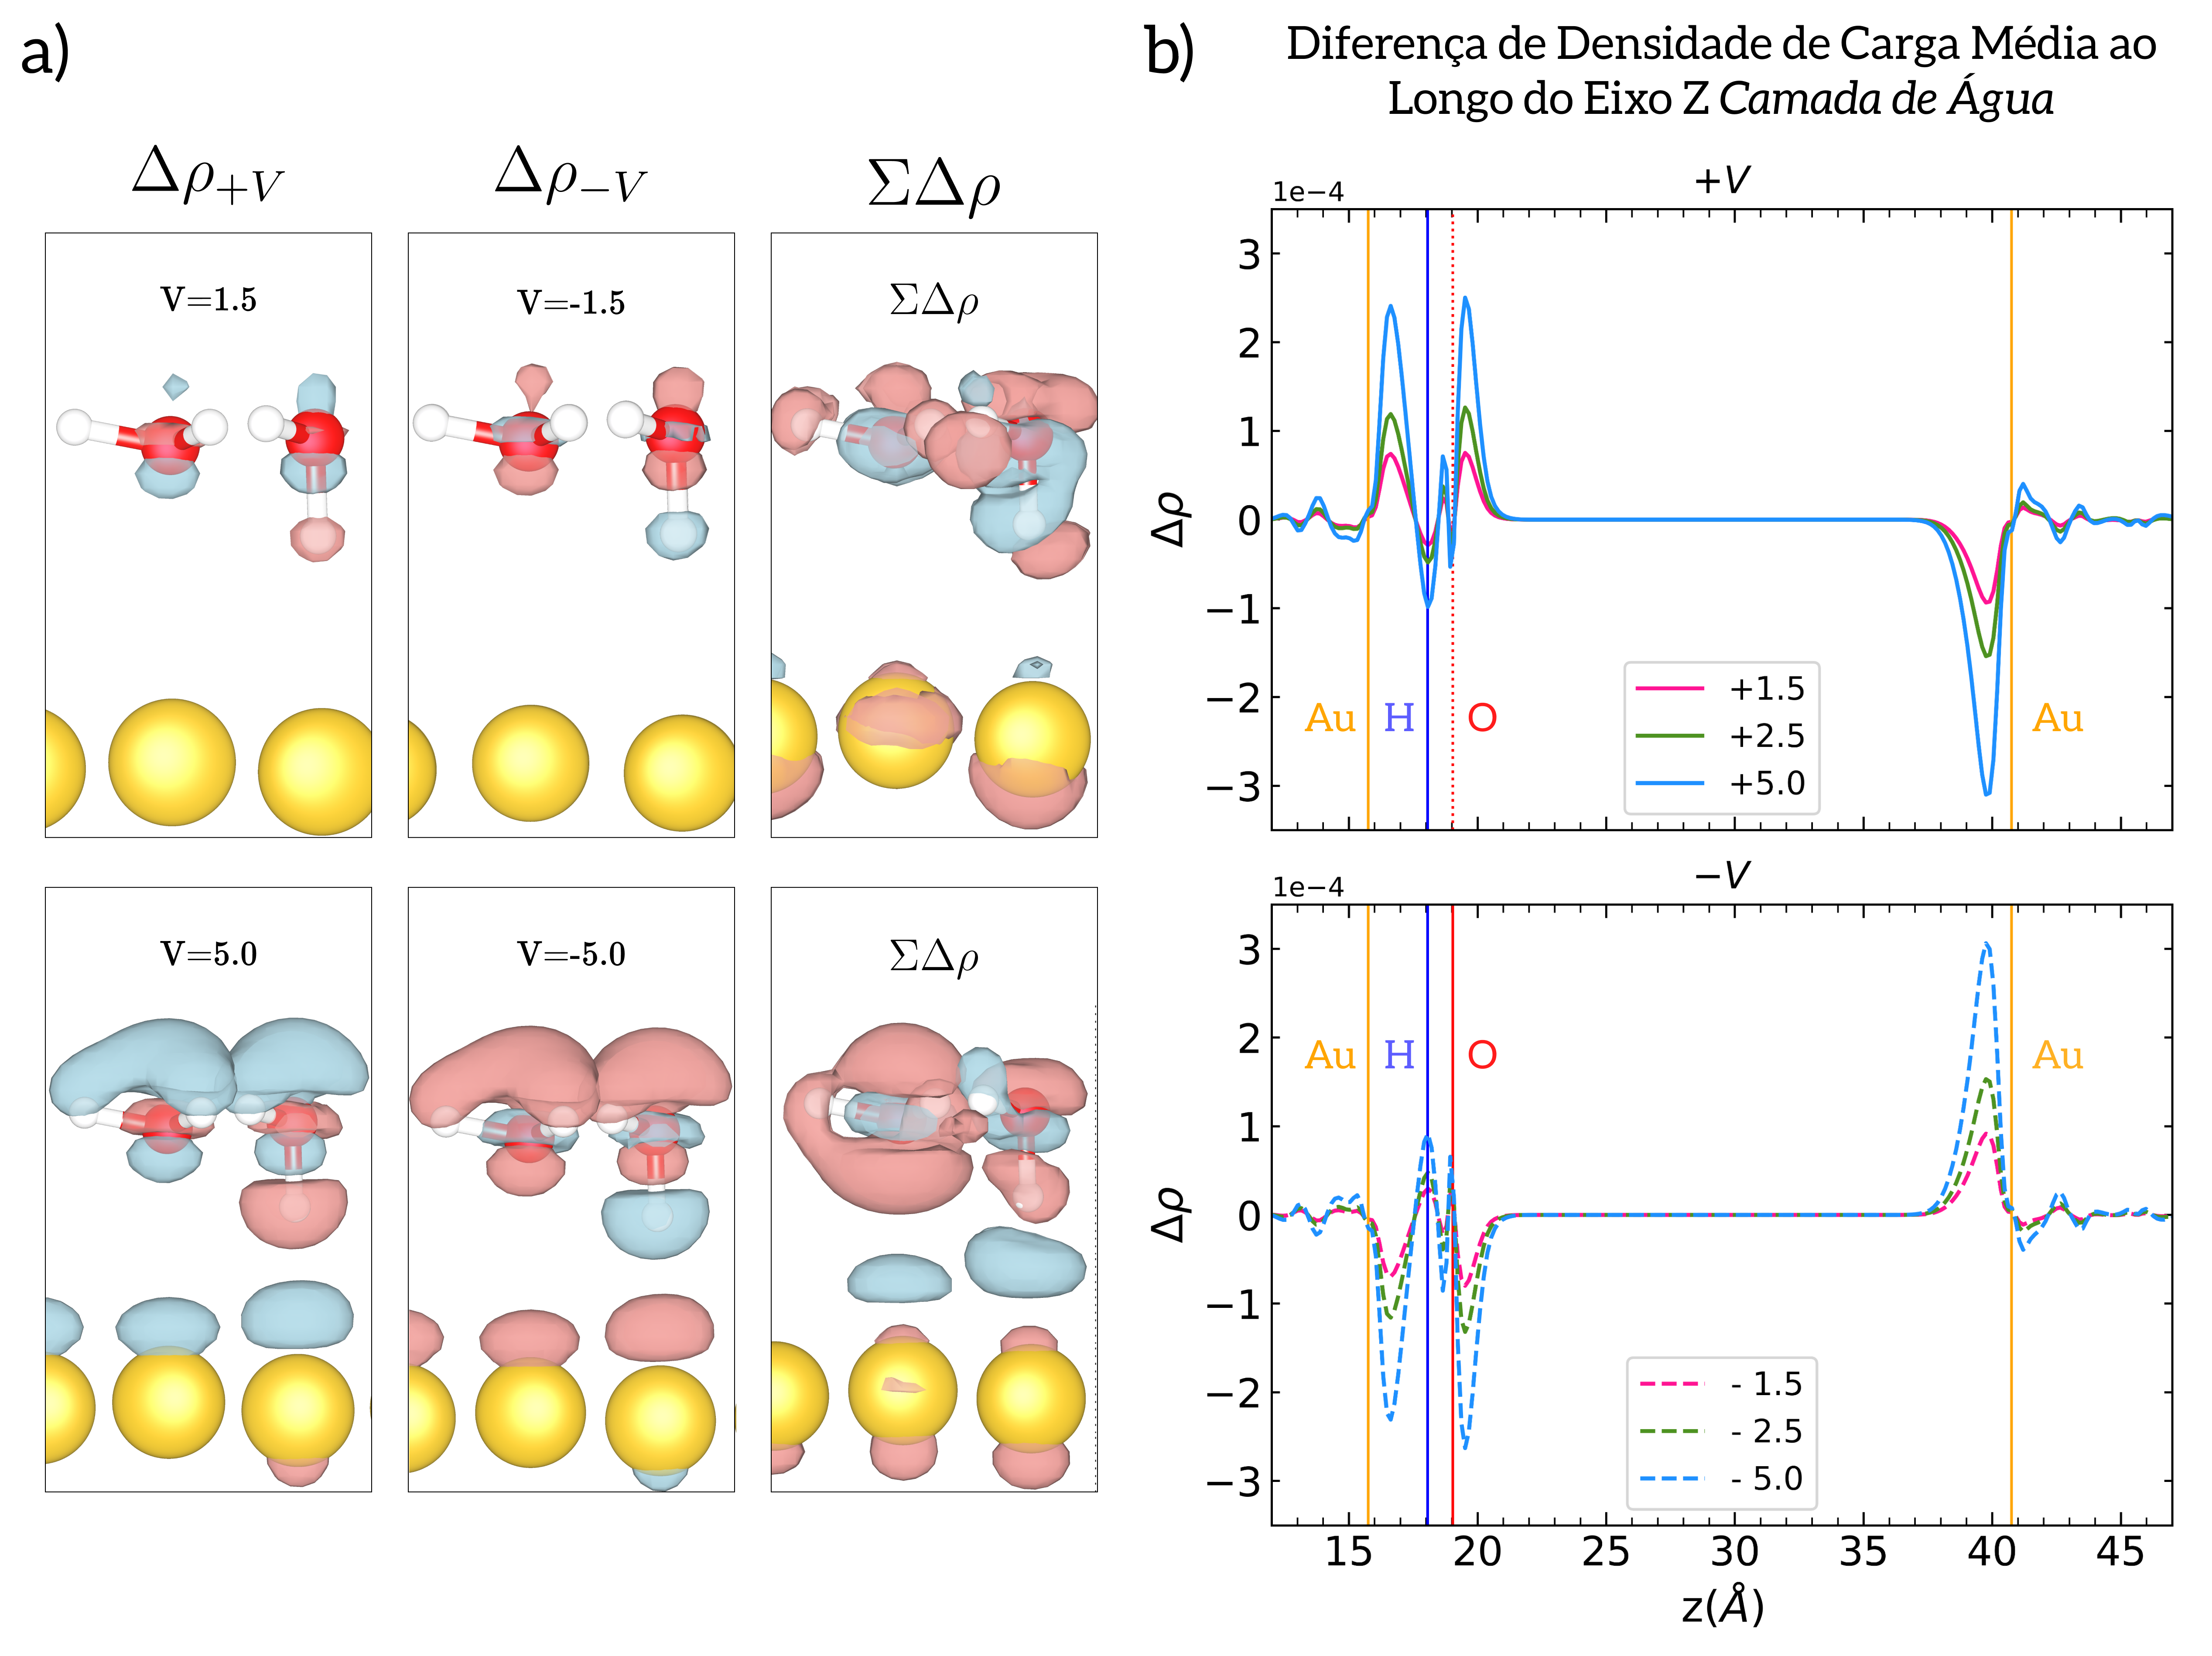
\includegraphics[scale=0.075]{figs/au_densidade_layer.png}
	\legend{Fonte: compilação da autora.}
	\label{fig:neq_au_dens}
\end{figure}

Dentre as propriedades geométricas, analisamos também as distâncias entre os átomos de oxigênio $ d_{OO1} $ e $ d_{OO2} $, no qual $ d_{OO1} $ refere-se às distâncias onde as moléculas \textit{flat-down} atuam como doadoras e $ d_{OO2} $ considera as distâncias onde as moléculas \textit{flat} que agem como doadoras (Figura \ref{fig:distancia_oo}). Assim, observa-se que para potenciais negativos têm-se uma maior variação das distâncias $ \Delta d_{OO1}=0.07\,\si{\angstrom} $. Para potenciais positivos essa distância se mantém praticamente constante, enquanto que $ d_{OO2} $ aumenta em até $ 0.04\,\si{\angstrom} $.


Para melhor compreender o efeito do potencial sobre as interações obtivemos os gráficos de diferença de densidade de carga e a média ao longo do eixo z -- Figura \ref{fig:neq_au_dens}. Através do gráfico de $ \Delta\rho_{_ {V}} $, observa-se que a concentração de densidade de carga está no átomo de O e que as variações de densidade e as transferências de carga são proporcionais ao potencial aplicado. Isso resulta na atração das moléculas \textit{flat} e \textit{flat-down} em direção à superfície metálica para V<0 e no comportamento contrário para V>0. Além disso, através da densidade média ao longo do eixo z, Figura \ref{fig:neq_au_dens} (b), observa-se que a transferência de carga entre as moléculas e o metal ocorre através da molécula \textit{flat-down} é maior. Isso é visto através da variação de carga que ocorre na posição correspondente ao átomo de hidrogênio próximo ao metal. %Através desses gráficos é possível também visualizar a interação entre as moléculas de água.% Por fim, observa-se .

Por fim, analisamos o efeito do potencial sobre as frequências dos modos normais de vibrações. Como o sistema é composto por 8 moléculas, então exitem 18 frequências fundamentais que foram representadas por uma distribuição normalizada (Figura \ref{fig:neq_au_freq}). Além disso, os valores superiores e inferiores das vibrações das frequências de \textit{bending} e \textit{stretching} estão representadas na Tabela \ref{tab:neq_freq_camada}. Através da projeção da densidade total de estados sobre as frequências vibracionais foi possível associar os picos às interações dominantes (interação água/água ou água/metal) e ao tipo de vibração (\textit{stretching simétrico ou assimétrico}). Assim, os valores representados na Figura \ref{fig:neq_picos} correspondem às frequências dos picos dominantes de acordo com a orientação da molécula responsável pela vibração dominante.

De modo geral, observa-se que as frequências inferiores estão associadas às vibrações de \textit{stretching} simétrica das moléculas \textit{flat-down} e correspondem à ligação O-H que participa da ligação de hidrogênio. Logo, essas ligações representam ligações O-H mais fracas, como pode ser visto pelo aumento da distância $ d_{OH} $, e ligações de hidrogênio mais intensas. As frequências intermediárias correspondem às vibrações de \textit{stretching} simétrica das moléculas \textit{flat} e de \textit{stretching} assimétrica das moléculas \textit{flat-down}. Essas últimas estão associadas às ligações O-H que interagem com o metal. As frequências maiores representam as vibrações de \textit{stretching} assimétrico das moléculas \textit{flat}. Além disso, observa-se que todas as frequências estão abaixo das frequências de \textit{stretching} assimétricos do dímero isolado.

Conforme o potencial aumenta negativamente, as frequências de \textit{stretching} tendem a se agrupar (Figura \ref{fig:neq_au_geo_layer}), de forma que os valores de \textit{stretching} inferiores aumentam e superiores diminuem -- Tabela \ref{tab:neq_freq_camada}. Além disso, observa-se pela Figura $\ref{fig:neq_picos}$ que as frequências das moléculas \textit{flat} tendem a diminuir, enquanto que as moléculas \textit{flat-down} aumentam. Esse resultado associado ao aumento da distância $ d_{OO1} $ da molécula \textit{flat-down} que atua na ligação de hidrogênio como doadora representa ligações de hidrogênio mais intensas e interações água/metal mais fracas. % Esse resultado condiz com observações experimentais nos quais mostram que a densidade superficial de água aumenta quando o metal está carregado positivamente e as frequências diminuem \cite{kramer} \cite{bibid}


Para potenciais positivos, observa-se uma dispersão das frequências, de forma que as frequências de \textit{stretching} superiores aumentam e as inferiores diminuem (Tabela \ref{tab:neq_freq_camada}). Além disso, observa-se um aumento das frequências assimétricas das molécula \textit{flat} e \textit{flat-down}, sendo mais proeminente para as frequências das moléculas \textit{flat-down}. Essas últimas estão relacionadas à interação água/metal e representa um enfraquecimento da interação água/metal. Ademais, o aumento nas frequência da molécula \textit{flat} refletem o crescimento da distância $ d_{OO2} $, de forma que as ligações de hidrogênio também são afetadas. 

%O modelo aqui analisado considerou o efeito do potencial externo sobre interações tipo água/água e água/metal. Através das propriedades analisadas, observa-se que  
\begin{figure}[b!]
	\centering
	\caption{Gráfico das frequências de \textit{stretching} características das interações dominantes de acordo com o potencial externo aplicado. As frequências foram separadas de acordo com a orientação da molécula (\textit{flat} e \textit{flat-down}) e pelo tipo de vibração (simétrico(S) e assimétrico(AS)). }
	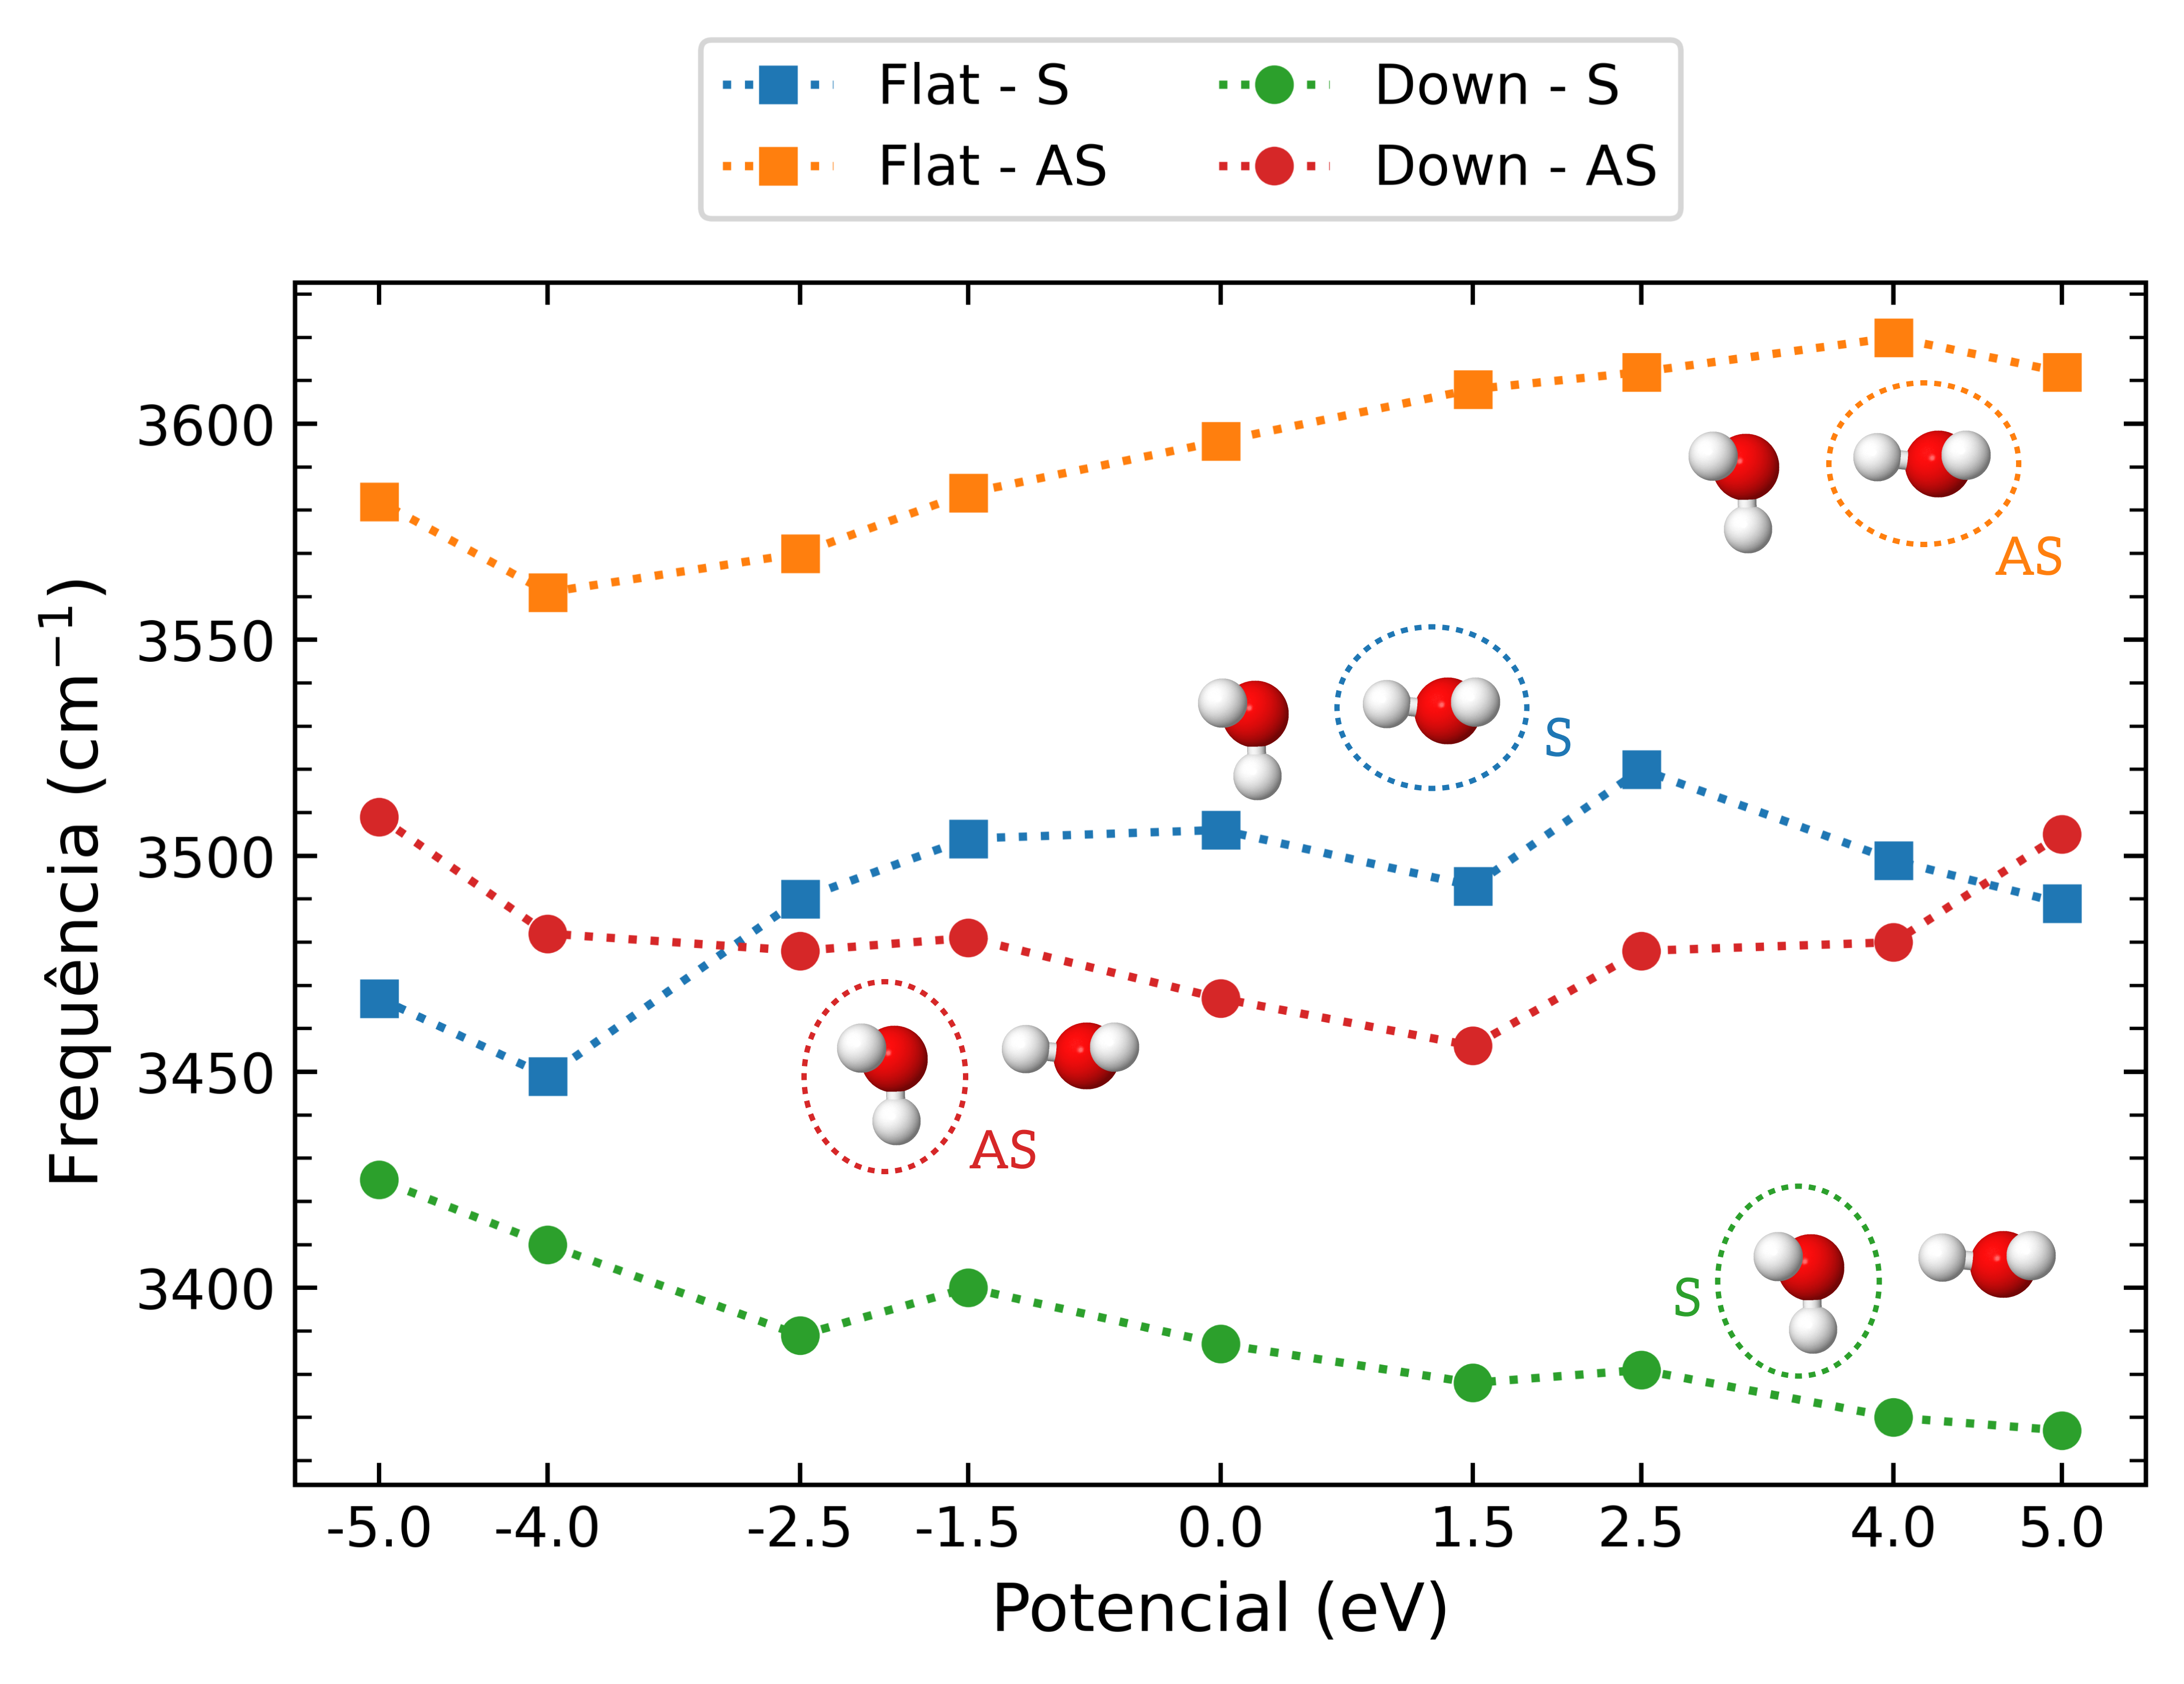
\includegraphics[scale=0.085]{figs/layer_picos.png}
	\legend{Fonte: compilação da autora.}
	\label{fig:neq_picos}
\end{figure}
Apesar do modelo estudado fornecer detalhes sobre  o efeito do potencial externo sobre interações tipo água/água e água/metal de uma camada de água, esse modelo não inclui interações das moléculas de água com a água \textit{bulk} ou o efeito do potencial sobre moléculas não-ligadas. Em particular, a presença da água \textit{bulk} é fundamental para compreender processos de oxidação e redução na superfície metálica carregada e têm sido investigada através da implementação de modelos contínuos \cite{bias_agua1,review_new}.  

Dessa forma, os resultados aqui encontrados mostraram que o potencial externo afeta principalmente as ligações de hidrogênio. Isso é visto pelas mudanças provocadas nas propriedades geométricas e vibracionais das moléculas \textit{flat}, uma vez que essas moléculas se aproximam do metal para potenciais negativos e se distanciam para potenciais positivos. Além disso, potenciais negativos intensificaram as ligações de hidrogênio, ao passo que potenciais positivos enfraqueceram tanto as ligações de hidrogênio quanto as interações água/metal. Por outro lado, através dos gráficos de $ \Delta\rho_{V} $ observa-se um excessos/deficiência de elétrons na região entre as moléculas \textit{flat-down} e o metal. Isso mostra que essas moléculas estão mais ligadas ao metal e portanto são menos afetadas pelo efeito do potencial externo.

 
\begin{table}[H]
	\centering
	\caption{Tabela contendo as principais frequências de vibração da camada adsorvida de acordo com cada funcional, bem como as frequências experimentais e teóricas do dímero isolado. \label{tab:neq_freq_camada}}
	\begin{threeparttable}
		\begin{tabular}{Scccccc} 
			\hline\hline
			\multicolumn{7}{c}{ \textbf{Frequências dos Modos Normais (\si{\cm}$ ^{-1} $) - Camada de Água} }                                                                                                                                                 \\ 
			\midrule
			{\multirow{2}{*}{V (eV)}}                                                  &  & \multicolumn{2}{c}{\textit{Bending }} &  & \multicolumn{2}{c}{\textit{Stretching}}                                                                            \\ 
			\cmidrule{3-4}\cmidrule{6-7}
			&  & Inferior & Superior                   &  & Inferior                                                 & Superior                                                \\ 
			\midrule
			-5.0                                                                     &  & 1616     & 1671                       &  & 3416                                                     & 3582                                                    \\
			-4.0                                                                     &  & 1621     & 1668                       &  & 3401                                                     & 3561                                                    \\
			-2.5                                                                     &  & 1622     & 1670                       &  & 3386                                                     & 3570                                                    \\
			-1.5                                                                     &  & 1623     & 1673                       &  & 3389                                                     & 3584                                                    \\
			0.0                                                                      &  & 1624     & 1672                       &  & 3369                                                     & 3596                                                    \\
			1.5                                                                      &  & 1625     & 1669                       &  & 3365                                                     & 3608                                                    \\
			2.5                                                                      &  & 1629     & 1668                       &  & 3365                                                     & 3612                                                    \\
			4.0                                                                      &  & 1633     & 1659                       &  & 3364                                                     & 3620                                                    \\
			5.0                                                                      &  & 1639     & 1656                       &  & 3353                                                     & 3612                                                    \\ 
			\midrule
			{Dímero Isolado~Exp.\tnote{$\dagger$}}&  & \multicolumn{2}{c}{1618.1}            &  & \begin{tabular}[c]{@{}c@{}}3547.5\\ 3697.7 \end{tabular} & \begin{tabular}[c]{@{}c@{}}3625.5\\3714.7\end{tabular}  \\
			\hline\hline
		\end{tabular}
		\begin{tablenotes}\footnotesize
			\item[$\dagger$]\citeauthor{ref-modos}
		\end{tablenotes}
	\end{threeparttable}
\end{table}





\begin{figure}[H]
	\centering
	\caption{Distribuição das frequências de vibrações ($\si{\cm}^{-1}$) das camadas de acordo com o potencial aplicado ($ \si{\eV} $). Os marcadores verticais representam os valores discretos das frequências. Além disso, está representado a interação dominante e a respectiva frequência; a linha tracejada representa as frequências experimentais do dímero isolado.}
	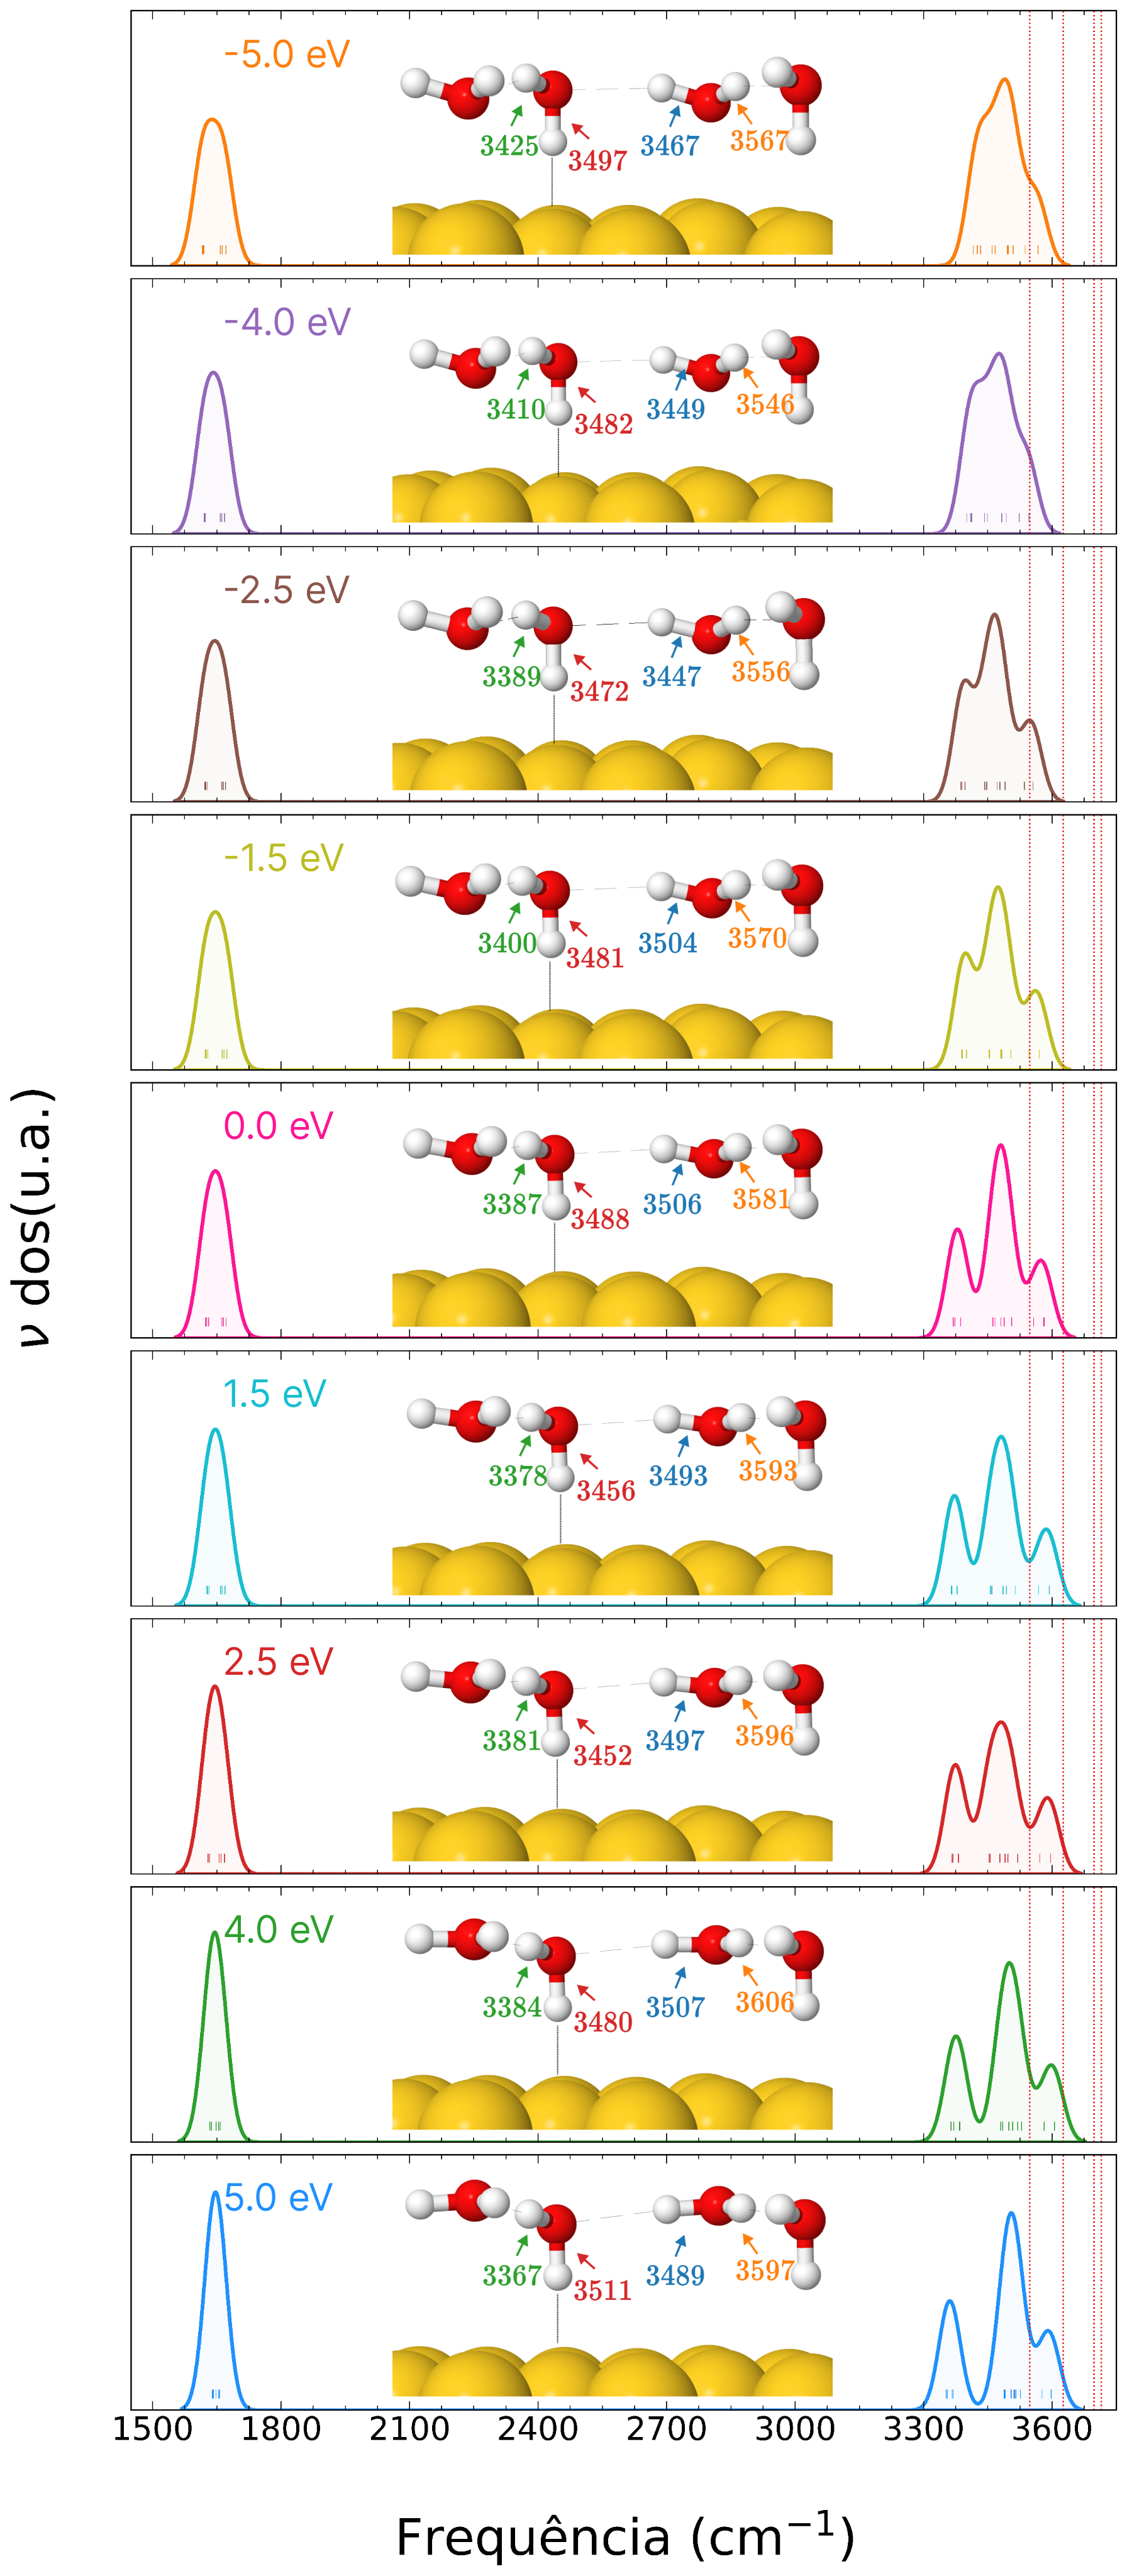
\includegraphics[scale=0.15]{figs/freq_layer.jpg}
	\legend{Fonte: compilação da autora.}
	\label{fig:neq_au_freq}
\end{figure}

